% Copyright (C) 2014-2016 by Thomas Auzinger <thomas@auzinger.name>

\documentclass[draft,final]{vutinfth} % Remove option 'final' to obtain debug information.

% Load packages to allow in- and output of non-ASCII characters.
\usepackage{lmodern}        % Use an extension of the original Computer Modern font to minimize the use of bitmapped letters.
\usepackage[T1]{fontenc}    % Determines font encoding of the output. Font packages have to be included before this line.
\usepackage[utf8]{inputenc} % Determines encoding of the input. All input files have to use UTF8 encoding.

% Extended LaTeX functionality is enables by including packages with \usepackage{...}.
\usepackage{amsmath}    % Extended typesetting of mathematical expression.
\usepackage{amssymb}    % Provides a multitude of mathematical symbols.
\usepackage{mathtools}  % Further extensions of mathematical typesetting.
\usepackage{microtype}  % Small-scale typographic enhancements.
\usepackage[inline]{enumitem} % User control over the layout of lists (itemize, enumerate, description).
\usepackage{multirow}   % Allows table elements to span several rows.
\usepackage{booktabs}   % Improves the typesettings of tables.
\usepackage{subcaption} % Allows the use of subfigures and enables their referencing.
\usepackage[ruled,linesnumbered,algochapter]{algorithm2e} % Enables the writing of pseudo code.
\usepackage[usenames,dvipsnames,table]{xcolor} % Allows the definition and use of colors. This package has to be included before tikz.
\usepackage{nag}       % Issues warnings when best practices in writing LaTeX documents are violated.
\usepackage{todonotes} % Provides tooltip-like todo notes.
\usepackage{hyperref}  % Enables cross linking in the electronic document version. This package has to be included second to last.
\usepackage[acronym,toc]{glossaries} % Enables the generation of glossaries and lists fo acronyms. This package has to be included last.
\usepackage{float}
\usepackage{appendix}


\newenvironment{conditions}
{\par\vspace{\abovedisplayskip}\noindent\begin{tabular}{>{$}l<{$} @{${}:{}$} l}}
	{\end{tabular}\par\vspace{\belowdisplayskip}}

% Define convenience functions to use the author name and the thesis title in the PDF document properties.
\newcommand{\authorname}{Rebeka Koszticsak} % The author name without titles.
\newcommand{\thesistitle}{Generating Expressive Window Thumbnails through Seam Carving} % The title of the thesis. The English version should be used, if it exists.

% Set PDF document properties
\hypersetup{
	pdfpagelayout   = TwoPageRight,           % How the document is shown in PDF viewers (optional).
	linkbordercolor = {Melon},                % The color of the borders of boxes around crosslinks (optional).
	pdfauthor       = {\authorname},          % The author's name in the document properties (optional).
	pdftitle        = {\thesistitle},         % The document's title in the document properties (optional).
	pdfsubject      = {Subject},              % The document's subject in the document properties (optional).
	pdfkeywords     = {a, list, of, keywords} % The document's keywords in the document properties (optional).
}

\setpnumwidth{2.5em}        % Avoid overfull hboxes in the table of contents (see memoir manual).
\setsecnumdepth{subsection} % Enumerate subsections.

\nonzeroparskip             % Create space between paragraphs (optional).
\setlength{\parindent}{0pt} % Remove paragraph identation (optional).

%\makeindex      % Use an optional index.
%\makeglossaries % Use an optional glossary.
%\glstocfalse   % Remove the glossaries from the table of contents.

% Set persons with 4 arguments:
%  {title before name}{name}{title after name}{gender}
%  where both titles are optional (i.e. can be given as empty brackets {}).
\setauthor{}{\authorname}{}{female}
\setadvisor{Dr. techn.}{Manuela Waldner}{Msc.}{female}

% For bachelor and master theses:
%\setfirstassistant{Pretitle}{Forename Surname}{Posttitle}{male}
%\setsecondassistant{Pretitle}{Forename Surname}{Posttitle}{male}
%\setthirdassistant{Pretitle}{Forename Surname}{Posttitle}{male}

% For dissertations:
\setfirstreviewer{Pretitle}{Forename Surname}{Posttitle}{male}
\setsecondreviewer{Pretitle}{Forename Surname}{Posttitle}{male}

% For dissertations at the PhD School and optionally for dissertations:
\setsecondadvisor{Pretitle}{Forename Surname}{Posttitle}{male} % Comment to remove.

% Required data.
\setaddress{Address}
\setregnumber{1325492}
\setdate{01}{01}{2001} % Set date with 3 arguments: {day}{month}{year}.
\settitle{\thesistitle}{Generating Expressive Window Thumbnails through Seam Carving} % Sets English and German version of the title (both can be English or German).
%\setsubtitle{Optional Subtitle of the Thesis}{Optionaler Untertitel der Arbeit} % Sets English and German version of the subtitle (both can be English or German).

% Select the thesis type: bachelor / master / doctor / phd-school.
% Bachelor:
\setthesis{bachelor}
%
% Master:
%\setthesis{master}
%\setmasterdegree{dipl.} % dipl. / rer.nat. / rer.soc.oec. / master
%
% Doctor:
%\setthesis{doctor}
%\setdoctordegree{rer.soc.oec.}% rer.nat. / techn. / rer.soc.oec.
%
% Doctor at the PhD School
%\setthesis{phd-school} % Deactivate non-English title pages (see below)

% For bachelor and master:
\setcurriculum{Media Informatics and Visual Computing}{Medieninformatik und Visual Computing} % Sets the English and German name of the curriculum.

% For dissertations at the PhD School:
\setfirstreviewerdata{Affiliation, Country}
\setsecondreviewerdata{Affiliation, Country}


\begin{document}
	
	\frontmatter % Switches to roman numbering.
	% The structure of the thesis has to conform to
	%  http://www.informatik.tuwien.ac.at/dekanat
	
	\addtitlepage{naustrian} % German title page (not for dissertations at the PhD School).
	\addtitlepage{english} % English title page.
	\addstatementpage
	
	\begin{danksagung*}
		\todo{Ihr Text hier.}
	\end{danksagung*}
	
	\begin{acknowledgements*}
		\todo{Enter your text here.}
	\end{acknowledgements*}
	
	\begin{kurzfassung} 
		Thumbnails werden benutzt um eine Liste von geöffneten Fenstern und Tabs anzuzeigen, wenn auf Computern oder mobilen Geräten zwischen ihnen gewechselt wird.
		Diese Bilder erleichtern das Erkennen der offenen Applikationen, und helfen, dass das nötige Fenster schneller gefunden wird.
		Thumbnails sind aber nur ein verkleinerter Screenshot von den Fenstern; wenn aber Tabs oder die selbe Applikation mehrmals offen sind, werden sie leicht unübersichtlich.
		Abhängig von der Auflösung des Bildschirms werden die Thumbnails kleiner, wenn die Anzahl der offenen Fenster steigt.
		Außerdem sind Screenshots von der selben Applikation sehr ähnlich, zum Beispiel die Seite und Toolbar in MS Office Word, der Text auf der Seite ist aber nicht lesbar. 
		Es gibt bereits mehrere Möglichkeiten, wodurch die beim Bearbeiten entstehenden Artifakte weniger auffällig und die wichtigen Regionen hervorgehoben werden können.
		In dieser Bachelorarbeit wird eine Applikation entwickelt, welche diese Methoden auf Screenshots anwendet und Thumbnails erstellt.
		Screenshots von Applikationsfenster werden durch eine Kombination aus Cropping, Abschneiden von irrelevanten Elementen an der Seite, Seam Carving, Verkleinern durch Herausschneiden unwichtiger Pixel-Pfade, und herkömmlichem Down-Sampling zu Thumbnails verkleinert. 
		Die Ergebnisse zeigen also nur relevante Informationen an, wodurch sie expressiver sind und ihren Zweck besser erfüllen können.
		
	\end{kurzfassung}
	
	\begin{abstract}
		Thumbnails are used to display a list of open windows or tabs when switching between them on computers
		and on mobile devices. 
		These images make it easier to recognize the opened applications, and help to find the needed window quicker. Thumbnails display however only a screenshot
		of the windows, so they get potentially confusing if there are more opened windows or if the
		same application is opened multiple times. Depending on the resolution of the display, the
		screenshot size decreases as the number of opened windows increases. Furthermore,
		within the same application (like MS Office World) the screenshots are similar in appearance
		(eg.~: white paper and tool bar), but the important text is not readable.
		There are several approaches that filter the important areas of the images to make editting
		less obvious or enhance the main region. In this bachelor thesis an application
		is implemented that uses these methods on the screenshots.
		Screenshots of windows are reduced by cropping the irrelevant elements of the margin area, by seam carving, thus elimination of non-importan pixel paths, and by common down-sampling.
		So the thumbnails show only relevant information,
		which makes them more expressive and easier to fulfill their purpose.
	\end{abstract}
	
	% Select the language of the thesis, e.g., english or naustrian.
	\selectlanguage{english}
	
	% Add a table of contents (toc).
	\tableofcontents % Starred version, i.e., \tableofcontents*, removes the self-entry.
	
	% Switch to arabic numbering and start the enumeration of chapters in the table of content.
	\mainmatter
	
	\chapter{Introduction}
	With the increasing use of mobile devices and reliance on multi-tasking thumbnails are becoming more important.
	Thumbnails appear when switching between tasks, representing the concurrent windows i.e. the running applications.
	To keep a continuous and effective workflow, it is essential to make the process of switching as fast and smooth as possible by allowing the user to quickly identify and choose between the given tabs and windows. 
	However, classic thumbnails are sometimes not sufficient for this purpose. 
	Due to the fact that standard thumbnail applications simply take the screenshot of each application and present them in a smaller size, the relevant parts of the window may no longer be recognizable.
	Figure~\ref{fig:thumbnails} shows the windows-switching tool of Windows 10.
	\begin{figure}[H]
		\centering		
		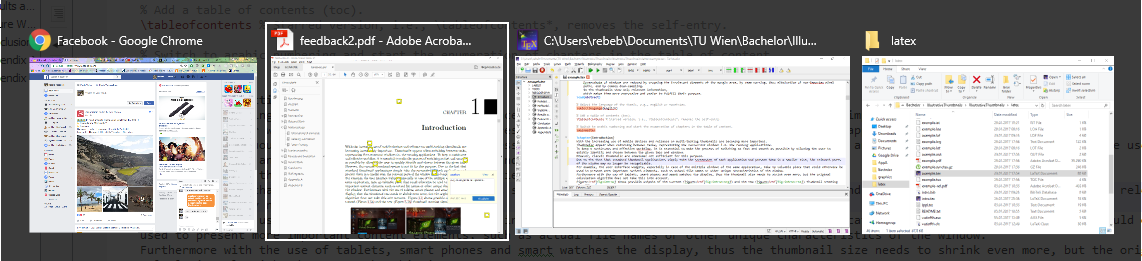
\includegraphics[width=\textwidth]{thumbnails}
		\caption{Visualization of the currently used thumbnail system on windows 10 in case of four running applications.}
		\label{fig:thumbnails}
	\end{figure} 
	For example, the user interface widgets, especially in case of the multiple windows of the same application, take up valuable space that could otherwise be used to present more important content elements, such as actual file names or other unique characteristics of the window.
	Furthermore with the use of tablets, smart phones and smart watches the display, thus the thumbnail size needs to shrink even more, but the original calculation algorithm does not take this into account.
	Figure~\ref{fig:introo} shows possible outputs of the current (Figure~\ref{fig:introo:org}) and the new (Figure~\ref{fig:introo:res}) thumbnail creating algorithms.\par 
	\begin{figure}[h]
		\centering
		\begin{subfigure}[b]{0.45\columnwidth}
			\centering
			
\includegraphics[width=\textwidth]{orgBlizzard}
			\subcaption{Classic thumbnail}
			\label{fig:introo:org}
		\end{subfigure}
		\begin{subfigure}[b]{0.45\columnwidth}
			\centering
			
\includegraphics[width=\textwidth]{resultBlizzard}
			\subcaption{Expressive thumbnail}
			\label{fig:introo:res}
		\end{subfigure}
		\caption{The result using the two different approaches.}
		\label{fig:introo} % \label has to be placed AFTER \caption (or \subcaption) to produce correct cross-references.
	\end{figure}
	%This project introduces a new approach using seam carving to make thumbnails more expressive even on small displays.
	Seam carving is a special re-sampling method, where seams along the least important image regions are eliminated to down-sample the image.
	The definition of importance depends on the implementation, but it in any case evaluates color changes and identifies the edges that shape the outline of the element on the source image.
	It is implemented for natural images, however, and not for screenshots, the usual saliency calculation is not adequate enough.
	Following a similar logic, the algorithm presented in this thesis uses the seam carving method, but it takes into account that the given input is essentially a screenshot.
	So it will probably contain some UI elements on the picture.
	Additionally, considering that letters are more common on computer screens than on usual images, the text content is also investigated to determine them as important regions.\par
	In summary, the thumbnail creating algorithm of this thesis performs cropping first to eliminate the UI elements of the margin area, then seam carving using a customized importance map and finally common down-sampling.
	While modified importance map is built from the usual saliency values of the screenshot and from the results of the text detection.
	
	%\section{Definition of the word illustrative} 
	To provide satisfactory results a detailed and clear definition of the word expressive is needed.
	Not only it influences the calculation of the pixel and region importance value, but also acts at the selection of result outputs, and is useful for future software development.
	Also, for a fitting definition it needs to be taken into account that in this case the seam carving algorithm is used for screenshots and not for usual photographs.\par 
	The expression 'expressive thumbnail' also comprehends that it is able to represent more information on a same sized picture than the other not expressive thumbnail.
	Unlike usual visual features observed on real world images, such as color changes and location of edges, as mentioned above, computer screens have additional special properties that require further consideration.
	For example, most screenshots include UI widgets, that are classified as not expressive in case of expressive thumbnail creation.
	Namely, it is rarely the case that the relevant part of an application is its UI and not its the actual content processing features, additionally, the identification of the a window in question is also possible by reading its title.
	Furthermore text data has on the computer screen more important role then usual pictures.
	To transmit as much information as possible, text data is not allowed to get damaged, i.e. even after size reduction it needs to stay readable.
	Figure~\ref{fig:textDamage} shows a possible output of the seam carving algorithm using different importance maps.\par 
	\begin{figure}[H]
		\centering		
		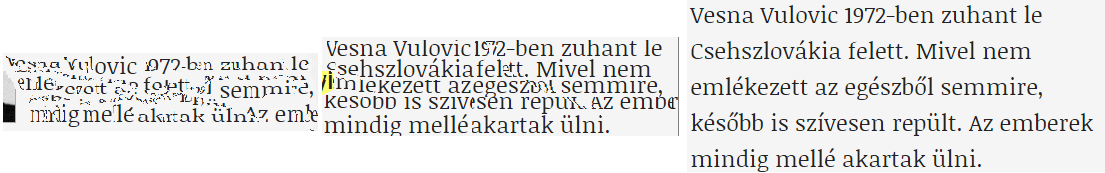
\includegraphics[width=\textwidth]{textDemage}
		\caption{The text damage using caused by seam carving using saliency map and modified importance map of this application. }
		\label{fig:textDamage}
	\end{figure} 
	Summing up, in this project a thumbnail is called 'expressive' if it preserves the information content.
	To measure this property, contrast values, color changes, location of edges, text data and the presence of UI elements are evaluated and considered.            
	
	\chapter{Related Work}
	There are several image processing algorithms that can be helpful at creating illustrative thumbnails.
	The main difference between these algorithms is whether they consider the input as an actual application window or just as a regular image.
	Therefore, this section is divided into two parts.
	The first one discusses algorithms with UI processing segments.
	Algorithms, invented for re-sampling natural images, are examined in the second section. 
	Moreover, there are two classes of information presentation methods are to be distinguished, namely, simple resizing and collages, the latter combining the most important parts of the image. 
	In the following, these methods are compared.
	
	\section{Processing as UI}
	When the input is a screenshot, there is a high chance that the usual UI elements, like buttons and menu bars, are shown on the screen.
	Exceptions for this are only cases when graphics, images, videos or application are presented, such as video games, gallery program or video players.
	Such applications tend to hide all UI elements and operate in 'fullscreen' mode, or use a redefined UI e.g. game menu bars.\par
	Labeling the image parts as content and non-content, the metadata about the UI elements can be helpful.
	Chang et al. ~\cite{chang2011associating} use already existing accessibility APIs, tested on Mac OS X and on Microsoft Windows, to segment UI and non-UI data. 
	Matching the metadata with the screen content provides a fast and robust result about the location of any kind of UI content.
	There are however several disadvantages, that need to be taken into account when using such APIs.
	The range and the granularity of the support is often not wide enough.
	The use of an accessibility API is unable to ensure that every UI elements are recognized, because some metadata are not reachable or they will be ignored by the application.\par
	Consequently, Prefab ~\cite{dixon2010prefab} uses prototypes. 
	In the database, models and  prototypes of common UI elements are saved.
	The (components of) UI elements are then matched with the prototypes from the database, allowing a consequent access to the predefined metadata.
	Since the Prefab system is able to split complex widgets to their constructing elements, the database does not need to be unnecessary big, though it is still able to cover the most common UI elements.
	Figure~\ref{fig:prototype} a possible entity of the Prefab database.
	\begin{figure}[H]
		\centering		
		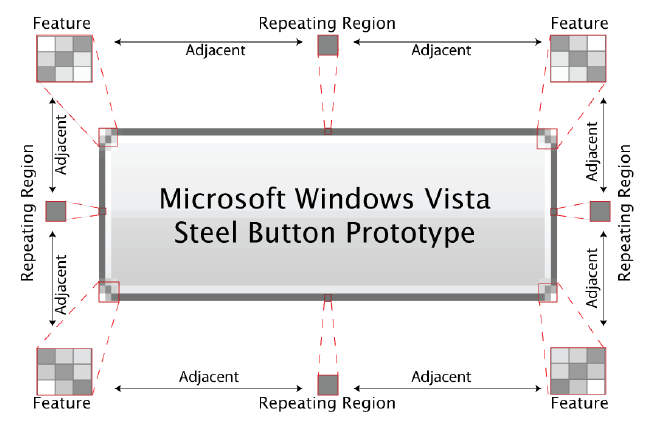
\includegraphics[width=0.5\textwidth]{prototype}
		\caption{Prototype of Windows Vista Steel Button in the Prefab database ~\cite{dixon2010prefab}}
		\label{fig:prototype}
	\end{figure} 
	In the case of special or rare UI widgets, like in a video game application or elements of a not widely used software, the system fails to recognize them, since these rare widgets are not included in the given database.\par
	Sikuli ~\cite{yeh2009sikuli} offers a solution not only for the incompleteness of such database, but for issues around granularity, too.
	It uses its own templates just like the Prefab system, but only in case of small icons and widgets.
	Since in case of larger objects template matching would be too expensive in terms of time and space, after accomplishing a training pattern, the Sikuli system is able to create new object models too.
	Although in the original application this feature is used for another purpose, i.e. to reduce matching costs, it can effectively used to solve the problem of database and granularity.
	With other words, Sikuli allows the expansion of the database and thus creating a more detailed database entries.\par	
	On the other hand, in case of accessibility APIs, it is not only the availability of the metadata that may cause problems, but also it does not provide information about the actual visibility of the UI elements.
	One window or rather one widget can overlap with or even fully cover another, some content can be out of the range of the borders of the screen etc.    
	The algorithm of Dixon et al. ~\cite{dixon2011content} is built on the Prefab system, but additionally it creates a hierarchical tree of the widgets. 
	The content is found at the leafs, and the parents are the widget, where the child is built in.
	With the help of this tree the order of the UI elements gets clear, and so the misleading information can be eliminated.\par
	After the labeling of the UI elements correctly, they can be manipulated as needed.
	They can cut off as whole or processed according to the information content.
	A UI widget can be highly detailed, where by resizing the originally smaller elements are no more recognizable or they interfere and take the space from each other. 
	Mirkamali et al. ~\cite{mirkamali2015object} invented an algorithm that eliminates the picture objects and fill their place with the texture of the object behind them using the z-buffer information.
	The tree mentioned above works as a z-buffer in this case.
	With this cut off algorithm, unnecessary widgets can easily be eliminated and more important elements, since they have more space, of the UI can thus get more visible.\par
	According to the definition of "expressive", the UI elements of a screen in any case are to be excluded, consequently the segmentation of the UI elements is not required.
	Although the Prefab and Sikuli systems are proved to be helpful at distinguishing between UI and content parts of the image, these approaches have their disadvantage at their reliance on database usage and at their slow template matching performance. 
	Furthermore they are actually designed for another purpose, namely to segment and classify UI elements, so before their employment significant reworking is needed.
	Since it is not essential to know, which exact widgets appear on the screen, and processing their actual content may cause performance issues, the use of the above methods would overcomplicate the application without providing noteworthy advantages.
	
	\section{Processing as a Regular Picture}
	There are several information saving methods for processing images with any kind of content.
	Furthermore, these methods can also handle a series of important tasks such as interesting point recognition, Region of Interest (ROI) selection, image or feature composition, i.e. tasks that are in order to make any kind of images more illustrative.
	Based on the type of input data, there are two groups of the above algorithms that will be discussed in the following sections.
	The first category works with more than one picture at the same time.
	Its strength is to choose single features that best represents the whole input data. 
	In exchange it is likely that no input image will be recognizable on the result.
	To the contrary, there are the methods in the second group that take only one picture for input and process it as one unit.
	The resulting image is similar to the input data, however thus it is likely that not only the unimportant but also the areas with high information ratio are damaged and also distortions may occur.
	
	%Finally, in the subsection below some approaches are presented that assist with the work of both of the above mentioned groups.
	
	\subsection{Collage Creating Methods} 
	A collage is an assembled image, containing parts of a bunch of input images and being representative for the whole input data.
	There are two cases by creating  more illustrative thumbnails where such methods can be helpful.
	On the one hand the actual information of a screenshot image is presented only in few regions of the picture.
	Many parts, for example UI elements, space between the content etc., can be ignored. 
	The other way around the content can be retrieved in form of ROIs, and afterwards they can be combined arbitrarily.
	On the other hand thumbnails for desktop switching can be easily generated using collage creator algorithms, where the input is screenshots of the open applications of the desktop instead of some ROIs of one screen.
	The following algorithms are implemented for natural images however, so in case of their use for thumbnail creation the methods need modifications accordingly.\par
	For a representative collage the most important task is to choose the best images, which information content covers the whole input data.
	Rother et al. ~\cite{rother2006autocollage} takes the parameters representativeness $E_{rep}$, importance costs  $E_{imp}$, transition cost  $E_{trans}$ and object sensitivity  $E_{obj}$ into account.
	\[ E(L)=E_{rep}(L)+w_{imp}E_{imp}(L)+w_{trans}E_{trans}(L)+w_{obj}E_{obj}(L) \]
	\[L = \{L(p), p \in \wp\}\]
	\[L(p) = (n, s)\]
	where:
	\begin{center}
		\begin{conditions}
			\wp & domain \\
			n & input image \\
			s & pixel-wise 2D shift of n \\
			w & adjusted weight by testing 
		\end{conditions}
	\end{center}
	Representativeness means being interesting in this case.
	A picture tends to have high representativeness value, if there are many special textures on it, and if it is not similar to the rest of the data (so that no image is chosen twice).
	Importance cost evaluates and collects the ROIs of the input.
	While transition cost stands for the smooth transition between every two images.
	At last, the parameter object sensitivity holds the results of object recognition, and it helps in the arrangement, that every object has a reasonable placement.\par
	Egorova et al. ~\cite{egorova2008collage} concentrates however only at the first two parameters above.
	It clusters the images according to their source and the time, and measures the quality.
	Thank to the clustering, by the choice of the final images it is clear,  which images are the same or have similar content.
	This feature, accordingly modified, can be useful by sorting ROIs of a screenshot, i.e.: text content, image content etc. or of the running applications of the desktop, i.e.: textprocessing, gallery application etc.
	The parameter quality summarizes the value of the results of the following calculations: blurriness, compression, contrast and color balance.
	Since in this case only screenshots, thus computer generated pictures, can be the input, these measurements invented for camera data would provide less meaningful results than the algorithm above.\par 
	\begin{figure}[H]
		\centering		
		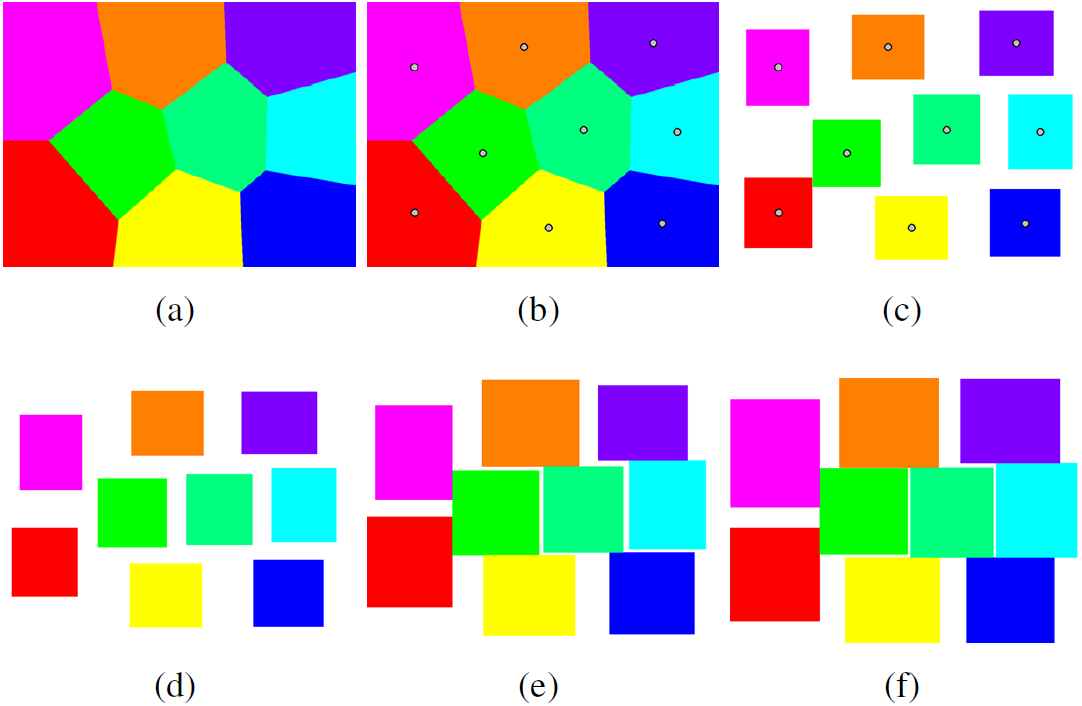
\includegraphics[width=0.5\textwidth]{ROIpacking}
		\caption{The whole ROI packing process ~\cite{lee2010mobile} (a) K-means clustering (b) ROI's center at the beginning of the algorithm (c) Layout of the ROIs at the beginning of the algorithm (d) Shifting of the ROIs (e) Expanding the ROIs (f) Output after some iterations}
		\label{fig:ROIpacking}
	\end{figure}
	Having the best ROIs for the collage the last task is to merge them into one output picture.
	For this purpose Lee et al. ~\cite{lee2010mobile} uses a method called ROI packing.
	First the central point of every ROI is selected and every pixel on the canvas needs to get assigned to one of them using the K-Means algorithm.
	After that the ROIs can be placed on the area calculated for them.
	To fill the place between the ROIs they are increased, keeping the aspect ratio, until they overlap. 
	Then every ROI is shifted to the middle of its area.
	This method is repeated until there are no further increases in the ROI anymore.
	To fill the white areas and eliminate any empty place, neighboring ROIs are allowed to partially cover each other.
	Figure~\ref{fig:ROIpacking} shows the different steps of the ROI packing algorithm.\par 
	Collage methods are excellent at representing a large image dataset in a small place.
	They work with numerous input data, take the most important parts of them and create a new image, that is not similar to any previous one.
	That is why they are more useful for making a thumbnail for a desktop while they do not necessarily provide as much advantages in case of applications.
	With taking the most important ROIs of one screen it would be possible to create a  more expressive image than any other, since the important content could stay large and so well readable, but classic collage assembly methods were developed for natural images. 
	These approaches need adjustment according to the different requirements for image and text regions.
	In one hand the collage method could minimize distortion of important regions since they stay rigid.
	In the other hand however, cutting a screen apart and arranging its parts willingly has a potentially confusing result for the user, requiring them to spend even more time with the screen recognition.
	
	\subsection{Re-sampling Methods}
	\label{relatedWork:resampling}
	To attain a constant relative position among regions, applying a resampling method is more effective than the above described collage creating approaches.
	Resampling means that some equally distributed parts of the image will be eliminated, thus, unlike by the collage algorithms, all remaining areas will have the same relation to each other.
	Therefore, the image itself remains recognizable because it has a highly similar appearance, in spite of having the most important areas less readable.\par 
	To select the invariable areas Chen et al. ~\cite{chen2003visual} suggests various attention models that are able to define the so-called Attention Objects (AO).
	AOs are usually real-world objects that due to their familiarity, shape, color etc., attract the human eye.
	AOs can easily be parametrized using three values: ROI, Attention Value (AV) and Minimal Perceptible Size (MPS).
	The attention models fit the AOs into their context.
	The algorithm works with three different attention models at the same time: saliency, face and text attention.
	The most important areas can be detected according to the importance value of each given pixel.\par 
	\begin{figure}[h]
		\centering		
		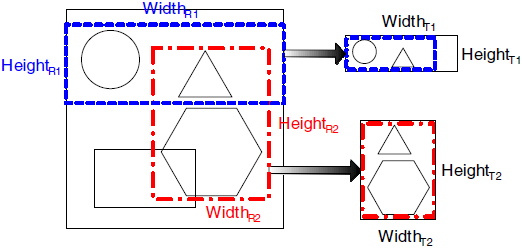
\includegraphics[width=0.5\textwidth]{useOfAOs}
		\caption{Possible solutions of the algorithm of Chen et al. ~\cite{chen2003visual}}
		\label{fig:useOfAOs}
	\end{figure}
	The approach above, after careful calculations, chooses the only area that contains the highest possible amount of AOs.
	To accomplish this, some possibly important AOs have to be ignored and cut off, as shown on Figure~\ref{fig:useOfAOs}.
	With feature-aware Texturing described in ~\cite{gal2006feature} this does not have to be the case.
	The algorithm expects an input image and a feature mask.
	A grid is generated, which lies on the input image.
	This grid can be modified into an optional shape, but the gridpoints on the feature mask are not allowed to change their proportion to each other.
	This way the picture elements between the AOs fill the new shape while the AOs get barely distorted, as illustrated on Figure~\ref{fig:fat}.\par 
	 \begin{figure}[h]
		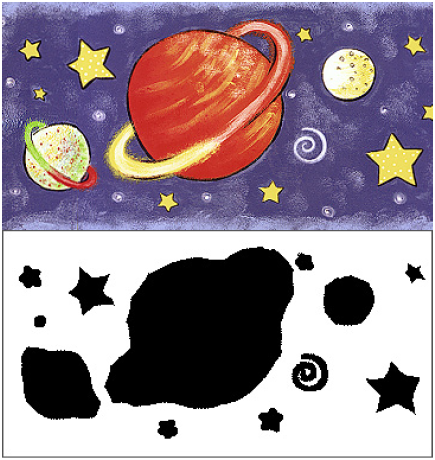
\includegraphics[width=.3\textwidth]{featureAwareTexturing1}\hfill
		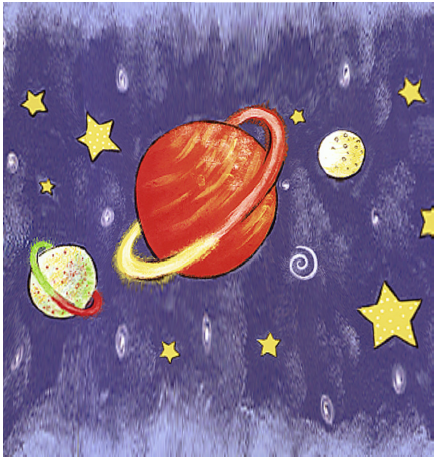
\includegraphics[width=.3\textwidth]{featureAwareTexturing2}\hfill
		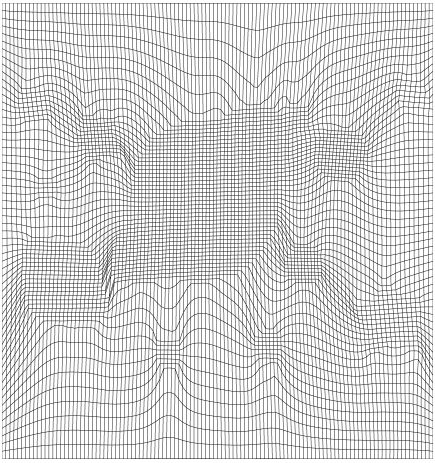
\includegraphics[width=.3\textwidth]{featureAwareTexturing3}
		\caption{The resulting image and grid from a certain input image and its feature mask of the Feature-aware Texturnig algorithm ~\cite{gal2006feature} }
		\label{fig:fat}
	\end{figure}
	A detailed importance is essential at creating thumbnails, since a screen usually contains a greater amount of sensitive information.
	Text data is not allowed to be ignored, so they need to be part of one or more ROIs.
	But the algorithms described above has aspects like face recognition and grid determination over-complicate the calculations.
	A face on a computer screen is not as frequent as on usual photos, and in addition it is not as sensitive as for example a text data.
	In the case of uniform down sampling a human face can stay recognizable, whereas texts quickly become illegible. 
	With a grid the input image can get reshaped to any other form with no additional damage to the important areas.
	But it is meant to form the input in completely other shape, not for resize it according to aspect ratio.
	Some aspects however, like definition of AOs, could expand the actual used approaches, this possibility will be discussed in the \hyperref[futureWork]{future work} section.
	
	\subsubsection{Seam Carving}
	\label{seamCarving}
	Seam Carving is a method, where unimportant pixel-paths are eliminated in order to down-sample the input image.
	Every pixel is first examined, how much information it contains, how important it is.
	After that horizontal and vertical seams, pixel-path where the following pixels are neighbors on the source image, can be calculated, and these with low importance value are cut off.
	With this approach the size of the input decreases without the loss a big amount of information. 
	Figure~\ref{fig:diff} shows the resized version of the same input using Seam Carving~\ref{fig:seamCarv} and simple down-samling~\ref{fig:downSampl}.\par 
	\begin{figure}[H]
		\centering
		\begin{subfigure}[b]{0.45\columnwidth}
			\centering
			\includegraphics[width=\textwidth]{AppB/game2}
			\subcaption{Seam Carved image}
			\label{fig:seamCarv}
		\end{subfigure}
		\begin{subfigure}[b]{0.45\columnwidth}
			\centering
			\includegraphics[width=\textwidth]{AppA/game2}
			\subcaption{Down-Sampled image}
			\label{fig:downSampl}
		\end{subfigure}
		\caption{The result using seam carving and common down sampling.}
		\label{fig:diff} % \label has to be placed AFTER \caption (or \subcaption) to produce correct cross-references.
	\end{figure}
	The importance map calculation depends on the individual implementation, but they are normally based on the saliency model introduced by Itti et al.~\cite{itti1998model}.
	Itti's saliency calculation takes the function of the low-level human visual system into account, so it pays attention for color, intensity and orientation of the pixels in the first row.
	In the calculation every pixel and its neighborhood is investigated, what relationship they have to each other.
	In this way the attention catching elements of an image, like color and intensity changes and lines or edges, can easily be found. 
	The architecture of this saliency model is illustrated on Figure~\ref{fig:salMod}.\par 
	\begin{figure}[H]
		\centering		
		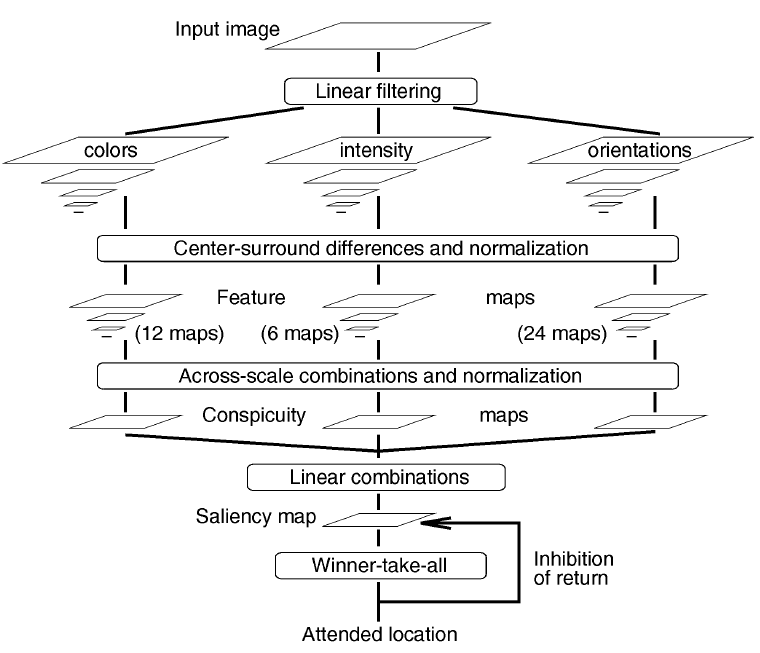
\includegraphics[width=0.5\textwidth]{saliencyModel}
		\caption{The architecture of the saliency model ~\cite{itti1998model}}
		\label{fig:salMod}
	\end{figure}
	According to the importance map Seam Carving is performed as by Avidan et al.\cite{avidan2007seam}, where the least important seams are simply eliminated.
	A seam runs from the top to the bottom or from the left to the right side and every pixel is part of the 8-neighborhood of the previous seam member.
	The final importance cost of every seam is calculated by summing up the importance value of the containing pixels.
	When this value is low, it means that the seam does not cross regions with high information content, so in case of elimination the data loss remains minimal.
	Figure~\ref{fig:seamsDol} shows the least important seams on a possible input image.
	Repeating this calculation, the image size can be reduces drastically without damaging the important regions as much as common down-sampling would do.\par 
	\begin{figure}[H]
		\centering		
		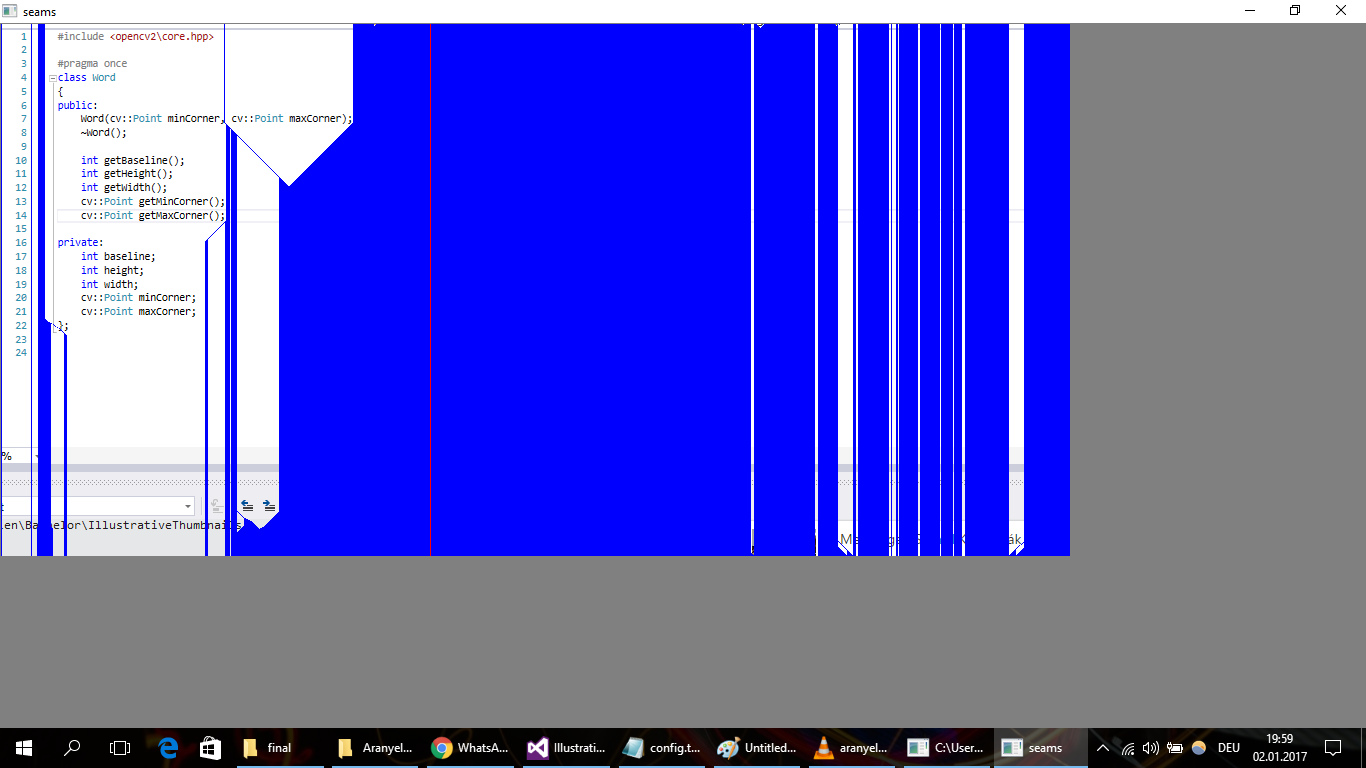
\includegraphics[width=0.5\textwidth]{seams}
		\caption{The least important seams of the image ~\cite{avidan2007seam}}
		\label{fig:seamsDol}
	\end{figure} 
	Since Seam Carving pays attention for the importance of one and other image regions by the creation of more expressive thumbnails is preferable over down-sampling.
	Seam Carving tries to save the high-information-content of the source, and eliminates only the non-relevant parts of the image.
	But how efficient it works it strongly depends on the importance map.
	In case of thumbnails, the calculation of the saliency is not sufficient, since it evaluates for example text data not as important as it finally should be.
	So in case of the use of Seam Carving for thumbnail creation the importance map calculation needs to get adjusted to the special requirements of a screenshot. 
	
%	\subsection{Feature combining methods}
%	All the above mentioned approaches work with some kind of feature combining algorithms.
%	After choosing the relevant areas that need to stay recognizable also on the resulting image, they are merged into one output picture according to their methods.
%	It is usual in this process  that some artifacts show up near the joining area.\par 
%	A possible solution for this problem is the Poisson equation for image processing, introduced by Perez et al. ~\cite{perez2003poisson}.
%	A modified Poisson equation using a guidance field needs to be solved for every color in the color space where the guidance field is calculated from the gradients of the input image.
%	This algorithm is actually invented for seamless cloning, but it is helpful when some not-neighboring parts of the same image need to be placed near each other.
%	To make the Poisson calculation more efficient an algorithm suggested by Hussain et al. ~\cite{hussain2016efficient} offers help.
%	It proposes to solve the equation with an image pyramid that is built from the source and the destination image, or, as in this case, from the two image regions to be combined.
%	To reach the most optimal result, Agarwala et al. ~\cite{agarwala2004interactive} works with gradient-domain fusion developed from the Poisson equation.
%	It collects the color gradients of the source images into a composite vector field.
%	Afterwards,  a color composition is calculated, where the gradient fits as well in the vector field as possible. \par 
%	Combining and accumulating the color data promises very smooth results with a natural appearance at the joining areas. 
%	These algorithms however are invented for combining pictures from the real world, and not for computer generated images.
%	In case of thumbnails, it is less important to make the transitions less edgy, since the source does not seem to be natural neater. 
%	So the use of such advanced methods like Poisson equation is pointless, since the offer, providing natural edges and smooth transition, matches not even the input screenshot. 
	
	
	
	\chapter{Methodology}
	\begin{figure}
		\centering		
		\includegraphics[width=\textwidth]{flowChart}
		\caption{Flow chart of the algorithm.}
		\label{fig:flowChart}
	\end{figure}
	The illustrative thumbnail creating algorithm has three main steps, as shown in Figure ~\ref{fig:flowChart}.
	At the beginning the UI elements are cropped.
	%In the case of thumbnails there are other ways to get information about what application are actually opened, for example by giving a title for it, containing the running application's name.
	It is rather usual that the same software is running multiple times, possibly for other purposes, e.g. using the text editor for both writing one and reading another document.
	The appearance of the applications is thus very similar, and they may no longer be discriminable when scaled down.  
	Consequently, the actual content and not the surface of these applications makes a difference.
	Although reading the title of the thumbnails may be slower than the software recognition through low-level visual data, this aspect needs to take count for the better visualization of the actual content area.%TODO{trade off} 
	The second step is the calculation of the importance map weighted by the location of text data.
	Unlike at regular real-life pictures the occurrence of text on computer screens is very common, and possibly is the main discriminating content.
	For this reason the calculation of the final importance map has two steps.
	First the importance value of every pixel is generated according to an image based energy function described in the next sections.
	Second the importance value is increased at the places where text is found.
	This way not only the silhouette but also the whole body of the letters and the space between them is marked salient. 
	Lastly, seam carving and simple re-sampling is performed  until the correct output size is reached.
	In this section these three main sections are discussed, and an overview of the algorithm is presented.	
	
	\section{Eliminating UI elements}
	For the elimination of UI elements, first their identification must be accomplished. 
	For the search of UI widget three heuristics were developed.
	The first one implies that these UI elements are located near the border of the screen and not in central areas.
	Secondly, it is assumed that the UI has similar background or theme color, and it differs from the rest of the window.
	Finally, the UI area is bounded by a straight line, while the horizontal one is longer than the vertical.
	Thus, the middle of the screen is taken as reference data for the investigation and is not checked for UI elements.
	The UI elimination algorithm operates right on the source window in the border area, which size is predefined and parametrized, i.e. no further premodification is required for this process.\par
	In case their order is relevant, while cropping the borders first the horizontal, then the vertical margins are investigated.
	The cropping algorithm, described in the following, is based on the assumption that upper and lower bars expand through the whole width of the display.
	The sidebars, if they exist, run however between the upper and the lower bars, and cover the remaining areas of the margin.
	Furthermore, occasionally the sidebar has a slightly different style than the other UI widgets mentioned above.
	The UI matching method investigates slices of the screen running along the margins; examining their color histograms determines whether they belong to the UI or to the middle area of the window.
	Because of the use of color histograms and the assumption that the UI has similar background color, which is different from the content, it is important to investigate a coherent data, so the slices should cover only UI or only content area, and not a mix of them.
	The above described process with an established order of margin cropping is fit for this purpose. \par 
	%Ennel a resznel kb 5 komment volt. ugyhogy lehez ezert kicsit szajbargos. de kb mindegyik mondatban volt vmiamit nem ertett... :D :D Haha nem baj legalább én is értem 
	To identify the best cropping line, indicating the edge where the UI meets the content area, a double validation method is performed.
	The first step evolves searching for a row of pixels in the border area, which size is configurable and predefined as mentioned above, located however near to the center of the source, having the same color and no interruption along the horizontal sides of the screen.
	It means, the length of the row is equal to the width of the source, it has exactly one pixel from every column which are actually taking place in one line on the input image.
	But this pixel row is not necessarily an actual line or edge of the image, it is only a horizontal path, where every member has the same color. 
	This method is based on the observation that toolbars often have a unicolor background, furthermore the UI is normally bounded by a straight line, where such a pixel row can easily be found, as the examples illustrate on Figure~\ref{fig:lines}.
	Therefore, the task is to find a horizontal pixel path, which has already passed the widget and icon location area, but still belongs to the UI area, i.e. it contains the background color or the line at the edge of the UI and content area.\par
	\begin{figure}[h]
		\centering		
		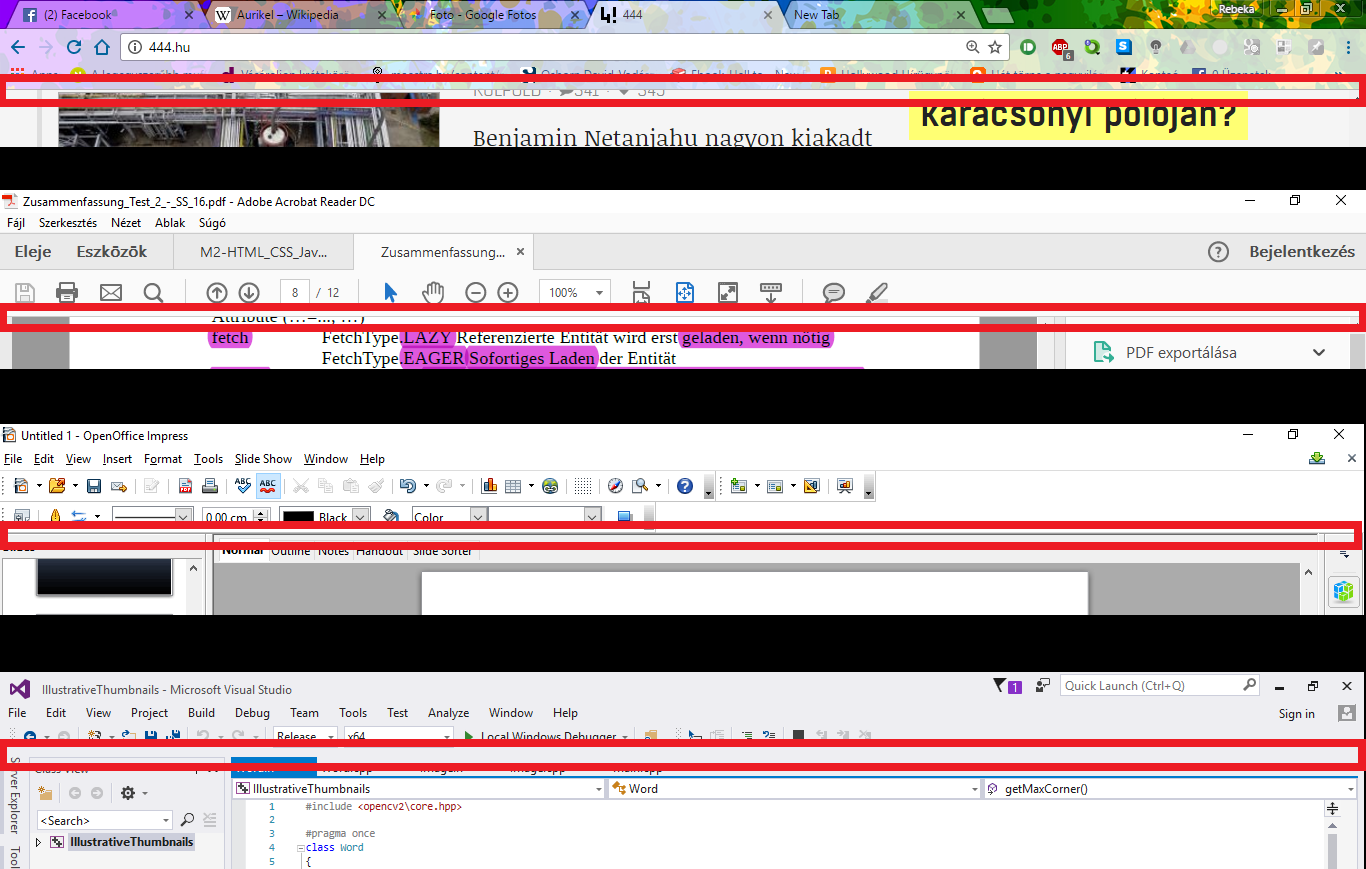
\includegraphics[width=\textwidth]{UIlines}
		\caption{Unicolor line at the edge of the UI area.}
		\label{fig:lines}
	\end{figure}
	In case of predefined UI areas the above method works well, on the other hand, there are several specific occasions where it is not able to provide any results.
	Outstandingly, game applications usually use their own graphical UI, but even at more traditional applications it is plausible that the UI area is so overloaded or designed that no background line can be found or the UI is simply not bounded by the edge mentioned before.
	For this reason it is important to perform an additional checking loop, too.
	This step is based on the correlation value of the border and center's color histogram calculated by the following equation~\cite{compareHist}:
	\[ d(H_{1},H_{2})=\left(\frac{\sum\limits_{J}(H_{1}(J)-H_{1})(H_{2}(I)-H_{2})}{\sqrt{\sum\limits_{J}(H_{1}(J)-H_{1})^2\sum\limits_{J}(H_{2}(J)-H_{2}})^2}\right) \]
	where:
	\[H_{k}=\left(\frac{1}{N}\right)\sum\limits_{J}H_{k}(J)\]
	\begin{center}
		\begin{conditions}
			N & Amount of the bins. 
		\end{conditions}
	\end{center}
	The result of this equation is between 1 and 0, if it is high it means that the two histograms are very similar, if it is low, however, it implies that they have no similarities.
	The margin is split into thin slices, where the actual size is parametrized and can be set as required, as a percentage portion of the actual height of the source.
	Initially the first slice near the border is examined.
	The histogram of this slice is then compared to the histogram of the center.
	If their correlation is high, where this threshold value can be defined, it implies that the two areas are not significantly different, therefore nothing should be cut off, and so the algorithm returns.
	Alternatively, if low correlation is found, the examined strips are not part of the same unit, indicating that the slice is supposedly from within the UI area.
	In this case, the two histograms, the one with the first slice and the other from the center region, are kept for reference values.
	In the next step, the remaining slices are compared with the two reference histograms, starting at the border and heading towards the middle area.
	Initially, the correlation with the border histogram is high and with the center is low, which shows that the slice is still in the UI area i.e. it matches the theme of the border widgets.
	\begin{figure}[H]
		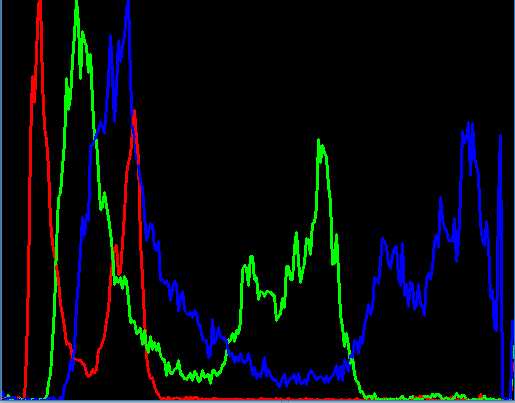
\includegraphics[width=.3\textwidth]{marginHist}\hfill
		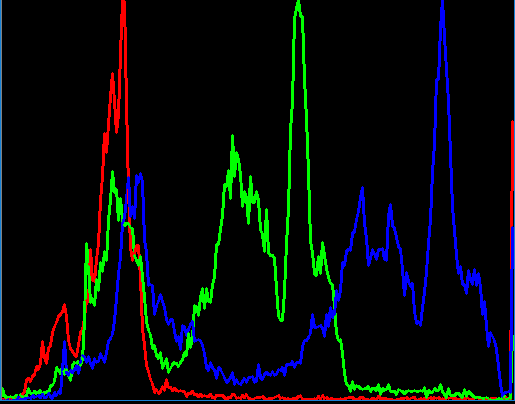
\includegraphics[width=.3\textwidth]{croppedHist}\hfill
		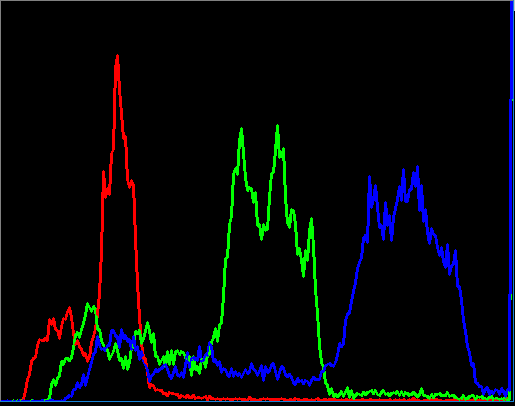
\includegraphics[width=.3\textwidth]{contentHist}
		\caption{The histogram of the margin area, of the slice, where the source~\ref{fig:cropped} is cropped and of the content region.}
		\label{fig:hist}
	\end{figure}
	This tendency reverses however as the slices approach the center regions.
	At the slice whose correlation with the center histogram is higher than the one with the border histogram, the algorithm stops, cuts all of the previously examined slices, and then terminates.
	Figure~\ref{fig:hist} displays the histograms of the margin, of the cropping and of the content area of Figure~\ref{fig:cropped}.
	Figure~\ref{fig:cropped} shows the borders between the content and UI regions found by the UI cropping heuristics.\par 
	\begin{figure}[H]
		\centering		
		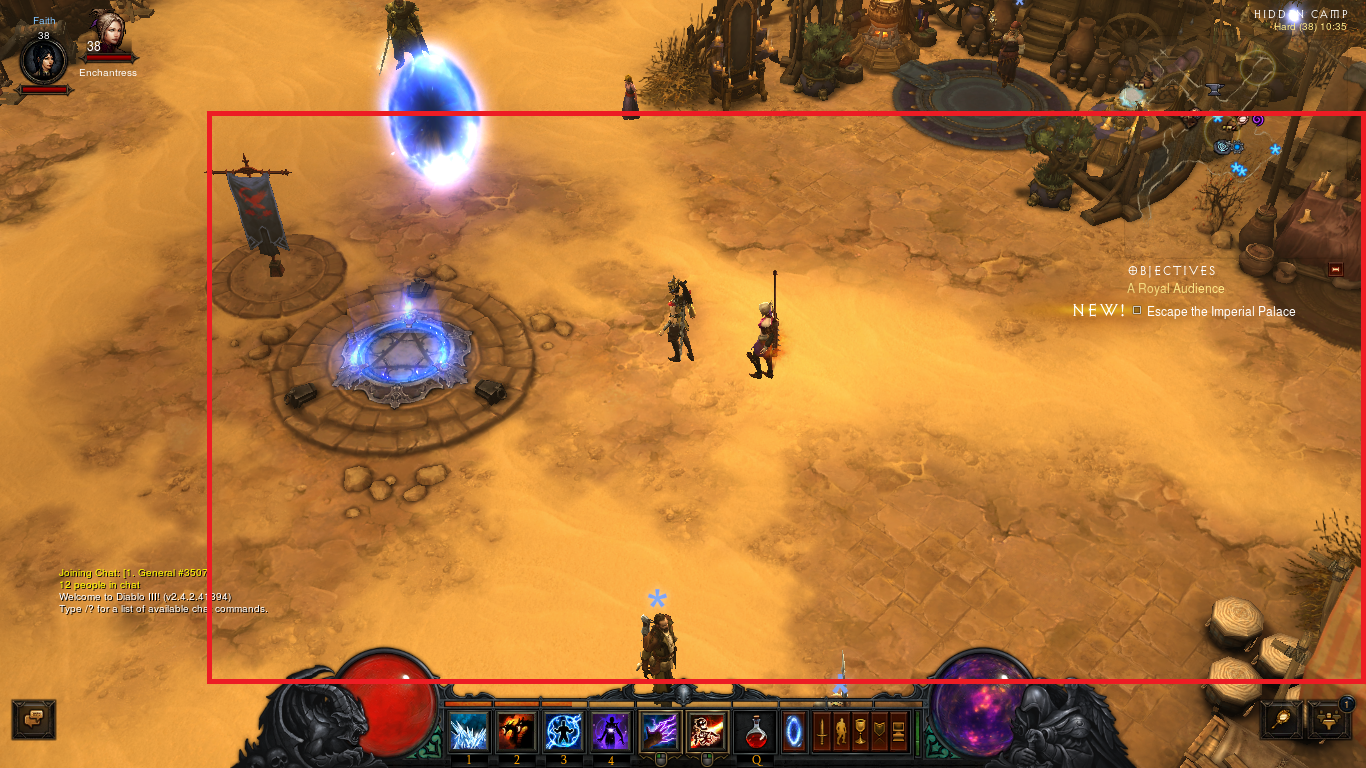
\includegraphics[width=\textwidth]{croppedGame2}
		\caption{The border of the content.}
		\label{fig:cropped}
	\end{figure}

	This method is executed four times.
	In the first two cases the upper and the lower borders are investigated.
	The third and the fourth loop are adjusted to the sidebars.
	In the first step, not a horizontal but a vertical line is searched, looking for a straight route, where the background color of the sidebar takes up the whole space between the already cropped upper and lower borders of the image.
	Finally, in the second checking loop the slices are defined vertically and not horizontally.
	
	\section{Importance Map Calculation}
	In order to ignore the parts of the source image that are actually unimportant, importance calculation is applied.
	The importance map calculation has two main steps: saliency calculation and text detection.
	In the following these two components of the algorithm is described.
	\subsection{Saliency Calculation}
	\label{saliencyCalculation}
	The saliency value of a pixel describes how much it stands out from its surrounding, how noticeable it is and how prompting it is for the human eye.
	A saliency map in this project is a matrix where the high value of an area means that the region is more salient than any other pixels with lower values.
	There are, however, many definitions and approaches about which pixels should be evaluated as salient or not salient, some of them is already mentioned in the \hyperref[relatedWork:resampling]{Related Work section}.
	In this case the saliency is calculated as presented by Niu et al.~\cite{niu2012image}. 
	There are two reasons, why this algorithm is chosen.
	First, it evaluates the low-level visual information just like the traditional method introduces by Itti et al.~\cite{itti1998model}.
	It means that only those pixels are valued as important that activate the low-level human visual system, for example due to their intensity or color change characteristics.
	In addition however, it is scale invariant, so it is more robust than other similar approaches mentioned before.\par 
	The algorithm converts the source into a perceptually linear, device-independent colorspace (Lu*v) first.
	After that, to make the approach scale invariant, a Gaussian contrast pyramid is built.
	The algorithm of Niu et al.~\cite{niu2012image} calculates the contrast value from the weighted sum of difference between the pixel and its neighborhood, using the L2 norm:
	\[ C_{i,j,l}=\sum\limits_{q\in\Theta}w_{i,j,l}d(p_{i,j,l},p_{q}) \]
	\[ w_{i,j,l}=1-\left(\frac{r_{i,j,l}}{r_{l,max}}\right) \]
	where:
	\begin{center}
		\begin{conditions}
			C & Contrast value \\
			(i, j) & pixel coordinates \\
			l & pyramid level \\
			\Theta & neighborhood \\
			w & weight \\
			d & difference \\
			p & color of the pixel \\
			r & distance from the image center \\
			r_{l, max} & maximum possible distance on the image.
		\end{conditions}
	\end{center}
	This approach needs to get slightly modified, in a way that the calculation ignores the weighting value.
	The weighting parameter is used because of the fact that the central area of regular real word images is more important than the margin regions.
	When investigating computer screens, however, this is not the case.
	A screenshot often does not have a defined focus point where the most important information is shown.
	By using the weighting value, the focus would be on the inner window, despite the fact that there is no actual significant correlation between the importance of the data and its position on the screen.
	The last step is to merge the contrast images into one complete saliency map.
	Upscaling of the levels is performed, so they have the same size to the cropped image.
	The pixel value of the saliency map is given from the sum of pixels with the same coordinates for every level of the contrast pyramid.\par
	
	\subsection{Text Detection}
	In the case of computer screens, texts are fairly common, and their information content is usually also very high.
	Therefore, it would be rather impractical not to reflect the importance of such text regions on the saliency map. 
	For that reason a further evaluation of the saliency map is needed, to check whether text areas were evaluated as important data.\par 
	The text detection algorithm is based on the one introduced in ~\cite{chang2011associating}.
	For the first step the whole input image is horizontally blurred, so that the letters and the neighboring words form a string together using connected component analysis.
	Thank to this blur operation very short words like "the", "a" or "I" do not get lost, because they will be connected to the words next to them.
	After that, all of these coherent strings are investigated and consorted depending on whether they are representations of actual words or if they derive from another visual feature of the source.
	The method that identifies the words examines two aspects.
	The first is if the strings are high enough but not too high to indicate real letters.
	Second, whether their width is not too small but also not too big to form at least one word but not an endless sentence.
	Both of these size examining values are parametrized, the thresholds can be set as needed, with their default value based on the size of one letter, in default case 5pt, as explained in the \hyperref[Implementation]{next chapter}. 
	The second loop evaluates the histograms of the area, where the strings were found.
	Normally the letters, if belonging to the same text data, have the same color, while the background, for optimal readability, does not change its color underneath the text, either.
	Therefore, the histograms of these areas are bimodal, meaning that they have one peak for the letters and one for the background color. 
	The two largest bins of the histogram are detected, and if they contain a predefined percent of the pixels, it is set for 65\% as default, then is the area labeled as actual word.
	To sum up, to identify a string as a word, it is not sufficient to pass the first check, it  also need  to have a corresponding special histogram. 
	Figure~\ref{fig:strings} shows the output of the text detection algorithm. 
	The light blue color labels the possible word regions, thus in the result of the connected component analysis the darker color denotes the actual words found by the algorithm.\par 
	\begin{figure}
		\centering
		\begin{subfigure}[b]{0.45\columnwidth}
			\centering
			\includegraphics[width=\textwidth]{444}
			\subcaption{Input image}
			\label{fig:strings:org}
		\end{subfigure}
		\begin{subfigure}[b]{0.45\columnwidth}
			\centering
			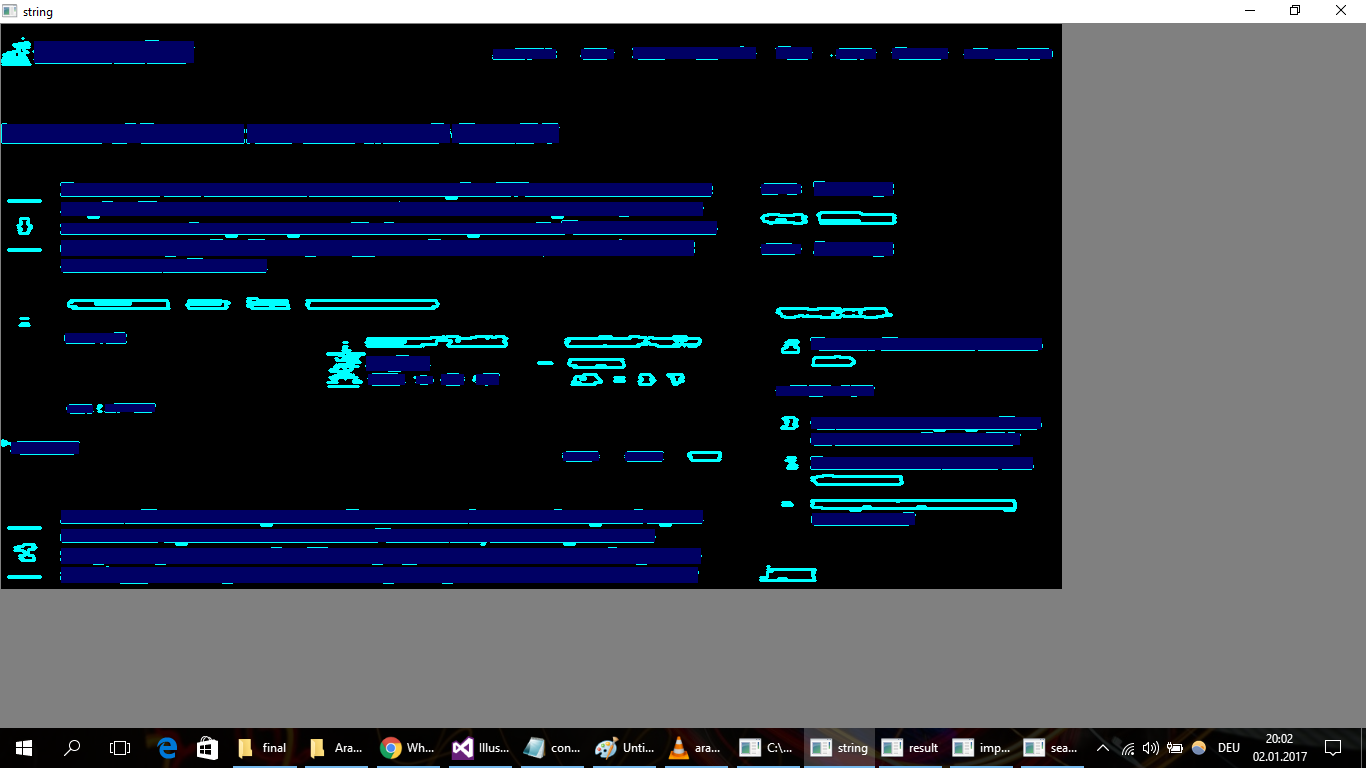
\includegraphics[width=\textwidth]{strings}
			\subcaption{Output}
		\end{subfigure}
		\caption{Result of the text detection algorithm applied on the given source.}
		\label{fig:strings} % \label has to be placed AFTER \caption (or \subcaption) to produce correct cross-references.
	\end{figure}
	The last step for the calculation of the final importance map, which is consequently used in the whole application, is to get the identified text regions weighted in the saliency map. 
	All areas that passed the word checking test are automatically evaluated as highly important, and get the highest saliency value in the importance map.
	In addition, to make sure that even the space between the words remains undamaged, which is important for greater readability, the area neighboring the text data is also weighted.
	Figure\ref{fig:saliency} is the final importance map of Figure~\ref{fig:strings:org}.
	\begin{figure}[h]
		\centering		
		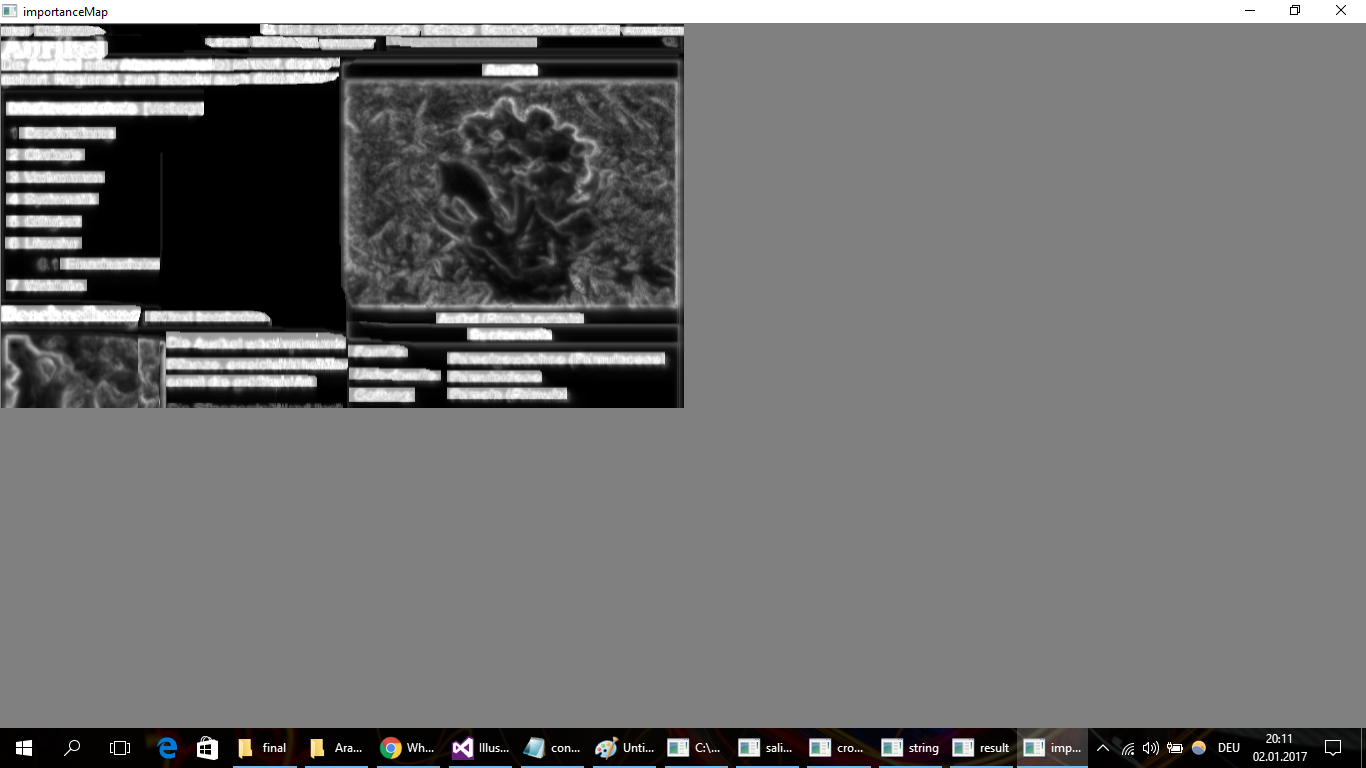
\includegraphics[width=\textwidth]{saliency}
		\caption{The final saliency map.}
		\label{fig:saliency}
	\end{figure}
	
	\section{Seam Carving}
	To resize the image without damaging the important regions, seam carving is used, mentioned in the \hyperref[seamCarving]{Related Work} section.
	Seam carving calculates paths according to the importance map, and eliminates those with minimal importance value.
	This step is repeated until the desired size is reached or the importance value of the chosen path exceeds a predefined threshold.
	Because seam carving does not necessary eliminate only the straight lines, the algorithm noticeably affects the layout of the unimportant regions.
	Furthermore, if the whole image has very high salient values, the resulting seams do not have a remarkably smaller salient value than any straight line would have had when chosen randomly for re-sampling.
	To save the image from unnecessary artifacts and to increase the application performance, a threshold indicating when to switch to re-sampling is defined, as Dong~\cite{dong2009optimized} proposed.
	To reach the final output size common down-sampling is applied.\par 
	To find the most appropriate path, every possible solution need to be examined using the backtracking method.
	A path map is thus generated, where all past possibilities belonging to the previous start pixels are stored, and where every new try that occurs when examining the next start pixel can be used as a look up.
	This way performance can be saved and the algorithm becomes faster.\par 
	To find the next pixel of the path, the five-neighborhood of the next possible member is examined.
	The algorithm runs from the top to the bottom, where the path to the next member is chosen from the five nearest pixels of the previous line.
	To calculate the costs of a possible switch between the columns the importance value of the neighboring pixels are weighted by $\sqrt{5}$, $\sqrt{2}$ and 1 according to their distance.
	In each case the chosen pixel is the one whose importance value with the weighting parameter is the smallest.\par
	Figure~\ref{fig:pathValues} is a visualization of the path map while running the algorithm.
	The yellow pixels are already set, the first row is automatically filled with the importance values from the importance map, the whites are however not known.
	The algorithm always takes the next unknown pixel running from left to right, from the top to the bottom and searches for an appropriate predecessor.
	The next point is displayed in the blue square.
	The possible predecessor of this point are shown in the red square.
	The importance of these pixels i.e. the yellow entities, saved in the path map, are compared, and the one with the smallest value is chosen.
	In case of the blue square pixel the coordinates of the chosen predecessor are stored and its importance value is set by adding the value in the predecessor pixel and the blue pixel value in the importance map together. 
	\begin{figure}[H]
		\centering		
		
\includegraphics[width=0.5\textwidth]{pathValues}
		\caption{Visualization of the path map in the middle of the calculation.}
		\label{fig:pathValues}
	\end{figure}
	Algorithm~\ref{alg:seamCarving} shows the flow of the seam carving process.
	Two paths per loop are calculated, one horizontally and one vertically, however, in the end only the pixels of the least salient path become eliminated.
	Additionally, since the output needs to hold the aspect ratio, in the end same amount of horizontal and vertical seams are eliminated. \par 
	\begin{algorithm}
		\KwIn{the cropped source image \textit{image}, the importance map of the cropped image \textit{saliencyMap}, two dimensional vector of the size of \textit{image} storing the saliency value and the previous path \textit{pathValues}  }
		\KwOut{seam carved \textit{image}}
		\While{\textit{y} < width of \textit{image}}
		{
			\While{\textit{x} < height of \textit{image}}
			{
				\textit{previousPixel} = detect the less salient pixel of the five-neighborhood in the previous line in \textit{pathValues} \\
				the saliency value of \textit{pathValues} at (\textit{x},\textit{y}) = \textit{previousPixel} + \textit{saliencyMap} at (\textit{x},\textit{y}) \\
				the path value of \textit{pathValues} at (\textit{x},\textit{y}) = position of  \textit{previousPixel}\\
			}
		}
		\textit{leastSalientPixel};
		\While{i < width of  \textit{pathValues} }
			{
			  Set \textit{leastSalientPixel} if the i-th value in the last row of  \textit{pathValues} is smaller than the value of \textit{leastSalientPixel}
			}
		\For{j = height of \textit{image}, j $\geq$ 0}
		{
			remove the pixel from \textit{image} with the coordinates of \textit{leastSalientPixel}\\
			\textit{lessSalientPixel} = the pixel in \textit{pathValues} with the coordinates of the path value of \textit{lessSalientPixel}
		}
		\Return(\textit{image})
		\caption{The seam carving algorithm}
		\label{alg:seamCarving}
	\end{algorithm}

	Because the horizontal and vertical paths are eliminated independently, the picture being processed usually does not hold the aspect ratio.
	For this reason it is plausible that the width and height parameters do not reach the output size or the threshold value at the same time.
	In this case the seam carving algorithm continues only for the remaining parameter, thus it is only looking for either horizontal or vertical seams, since the width or the height already hit the preconditions, until it reaches one of the conditions above. 
    The value of the threshold parameter is essential,	since it determines when the algorithm is to switch between seam carving and re-sampling. 
	It is calculated from the maximum salient path found after the first loop of the seam carving algorithm.
	This threshold value is further customizable, the different outputs in case of varying its value is discussed in the \hyperref[res:resampling]{Results and Evaluation} section.
	Since with every loop one unsalient pixel is eliminated from the horizontal or from the vertical path, the relative saliency of the seams constantly increases.
	Therefore, in most cases, even the least salient seam will get more salient than the most salient seam of the original image. 
	The common re-sampling method eliminates straight lines chosen from the source image until the desired size is reached.
	Seam carving is applied to prevent paths with high salient value to be cut off.
	On the other hand, if the seams have as high importance value as any other of the source image, regular re-sampling has additional advantages.
	First, the algorithm is faster than the implemented seam carving method, and second, it applies an interpolating algorithm between the borders of the eliminated area, so in this case it ultimately saves more information than seam carving.   
	
	\chapter{Implementation and Working Pipeline}
	\label{implementation}
	The expressive thumbnail creator application is developed in the programming language C++.
	Except for the source image file browsing window, no operating system specific calls are performed.
	To make the application platform independent in the future, only this part needs customization.
	For image processing purposes Open Source Computer Vision Library (OpenCV) is used ~\cite{opencv_library}.\par 
	Apart from being a computer vision library openCV is a machine learning library too.     
	It has more than 2500 algorithms that can be used for image processing or for machine learning tasks, among object identification, finding similar images, image stitching and so on.
	Since the library offers support not exclusively for Windows, but also for Linux, Mac OS and Android, all methods taken from OpenCV can be regarded as platform independent functions.
	The library is applied when loading and saving the images, and to perform several image processing tasks like converting between color spaces, and image editing task such as blurring or filtering.
	The actual use of the library is discussed in this section.
	Apart from the functionalities mentioned in the previous chapter, other vital helper methods are also discussed.
	To make the application configurable some essential parameters are set outside the source code. 
	The application uses a \texttt{config.txt} file, where every parameter can be set as needed.
	A list of these parameters are highlighted below.\par
	
	\section{Image Loading}
	Preceding the start of the thumbnail algorithm it is essential to load the source image.
	The application is not able to capture screenshots, it only reads the already saved screenshot image.
	To make the application more flexible a Windows call is performed, allowing a new source image to be chosen after each start of the application.
	The type \texttt{OPENFILENAME}~\cite{openfilename}, part of the Windows API, launches a file window to browse the required file.
	It shows only image files with the extension \texttt{.jpeg} or \texttt{.png}.
	After choosing the preferred source, the file path is established and the OpenCV function \texttt{loadImage} opens the picture.
	
	\subsection{UI Elimination}
	The default value of the border area is 20\% of the size of the sourec. 
	Starting from the border towards the direction of the middle of the source, every row and after then, every column, are searched for a specific source line that first, has the same color and second, a completely filled space between the vertical - later the horizontal - borders.
	Once accomplished, the OpenCV methods \texttt{rowRange} and \texttt{colRange} cut the input image.
	After cutting, the histogram of the remaining margin area is examined and compared to the central region, the margin is split along the nearest border into thin slices.
	The function \texttt{calcHist} calculates histograms of the marginal and of the central window.
	The function \texttt{compareHist} measures the correlation of two histograms.
	If according to it they do not correlate, the comparison is performed on other slices that are consequently labeled as margin or central windows.
	If a slice is found that correlates with the margin histogram, the image is cropped by the slice again. 
	The parameters of correlation and the width of the slices are also configurable.
	According to testings, the best results are provided when the correlation is between 1.3 and 2 and the width of the slices is the 0.25\% of the window.
	
	\section{Saliancy Map Clculation}
	The saliency map is calculated from a Gaussian pyramid.
	But before building the pyramid the cropped source image has to get converted into a uniform colorspace.
	For this purpose the OpenCV function \texttt{cvtColor} is called.
	Then the levels of the pyramid are determined using the \texttt{pyrDown} method.
	Afterwards a contrast map is calculated with the L2 norm using the equation mentioned in the \hyperref[saliencyCalculation]{Methodology} section from the four neighboring pixels for each level.
	In order to avoid any overflow, by merging the levels into one saliency map, the pixel values are divided by the amount of pyramid levels.
	
	\section{Text Detection}
	To find as many words as possible, the grayscale cropped source image is processed with the Laplacian operator, with the kernel size of three.
	The operator calculates the second derivate of the intensity values.
	In case of edges, there is an intensity change between the neighboring pixels, so the result of the Laplacian operator is zero and it indicates the edges.
	In that way the layout of the letters are now highlighted.\par 
	To make the series of letters related to each other, a horizontal blur is applied.
	The function \texttt{blur} is called. 
	Although its kernel size is configurable, by default the height is set to one, the width to 15 pixels. 
	Finally, the OpenCV function  \texttt{findContours} identifies the connected regions and saves their silhouette points into a 2 dimensional \texttt{vector}.
	For each region the bounding rectangle is calculated.
	If a region is at least double as wide as high, the function proceeds with the examination of these attributes, namely whether they reach the minimum size for being an actual word.
	The size of the minimal word is configurable and by default set to 5x5, approximately the font size of 5pt, in order to be able to take even the smallest fonts into account.
	In case a region passes the test, it is marked as a possible word and is forwarded for further investigation.\par 
	After labeling every region as word or non word region, the average height of the possible words is calculated.
	If the height of a possible word is according to a threshold smaller or greater than the average, it is automatically sorted out.
	This confidence interval is also configurable and it is set to 50\% and 1000\%. 
	The maximal word height is defined generously in order to be able to find also the potentially large-sized titles and headlines.
	The smaller words are however allowed to be sorted ot.
	On the one hand, if they are written so small, they information content is not as important as for example a headline.
	On the other hand, it would be difficult to preserve them readable, and they would take space from other content.\par 
	After the height test, the histogram of the possible word regions is examined.
	If it has exactly two accumulations, one for the color of the letters and one for the background, the region stays in the group of possible words, otherwise it is sorted out.\par
	Finally, the space above and below the possible words is investigated.
	Words are usually written in lines, with some space for readability placed between them. 
	Therefore if two possible word regions overlap i.e. have  common points at the top or at the bottom, it is inconceivable that the region in question represents a real words and thus is sorted out of the word list.\par 
	When the final list is ready, the regions of the words are to be marked on the saliency map.
	The value of every text data pixel is automatically increased to the maximum value.
	At the very end the whole map is normalized with the OpenCV function \texttt{normalize} to avoid value overflow by visualization and other irregularities.  
	
	\section{Seam Carving}
	Seam carving is implemented only in one, vertical, direction. 
	To be able to eliminate not only vertical but also horizontal seams, the cropped source image and the saliency map is rotated by 90 degree with the functions \texttt{transpose} and \texttt{flip}.
	For every loop a vertical and a horizontal seam is calculated, and the one with smaller saliency value is cut from the cropped source and from its saliency map.
	Until both sides reach the re-sampling value or the desired output size the seam carving algorithm is executed.\par 
	The re-sampling value is calculated from the average pixel saliency value of the most salient seam on the cropped source image.
	The desired size and the re-sampling parameter are both customizable, they are set by default to 50\%.
	At that point the algorithm have already switched to down-sampling usually.
	But by bigger size the differences are easier recognizable, and further down-sampling can be performed in any time.\par   
	The seam calculation algorithm works by writing a path map, where the previous paths and their saliency values are saved.
%	At the beginning, the first row of the map is filled with the saliency values of the importance map.
%	Afterwards, for the next row the least salient predecessor of every pixel is searched, and the saliency value at the coordinates of the current pixel is increased with the predecessor saliency value.
%	If the new saliency value is smaller than the one already stored at the coordinates of the current pixel, then the entry is updated and thus a better path is saved.
%	By looking for the predecessor pixel the algorithm works with 5-neighborhood. 
%	The saliency values of the five nearest pixels are weighted  by their distance form the current pixel with the values $\sqrt{5}$, $\sqrt{2}$ and one.
%	The pixel that is finally the least salient is chosen as predecessor.
%	When the algorithm finishes, in the end row of the path map the saliency values of the possible ways for starting at the first row are stored.
%	The final task is to find the smallest saliency value, and to follow the predecessor entities starting at the least salient pixel until the first row is reached again.
	The identified seam is afterwards eliminated not only from the cropped source image, but also from its saliency map.
	But if the saliency value of even the least expensive seam exceeds the re-sampling value, instead of cutting the path off, the usual re-sampling algorithm is applied using \texttt{resize} and the algorithm terminates.  
	
	\chapter{Results and Evaluation}
	In order to find the configuration, which provides reasonable results in as many cases as possible, several tests were performed.
	There is a test database including 14 pictures, showing seven different applications, captured on Windows 10.
	The test images and the results in case of the use of the recommended \texttt{config} file and the experimental results on Linux are listed in \hyperref[AppA]{Appendix A}. 
	In the following the test cases of the elimination of UI elements, text detection and for the value of re-sampling threshold are presented and evaluated in respect to which of them is best able to provide the desired results.
	Then the application is compared to Adobe Photoshop~\cite{photoshop}, with their advantages and disadvantages are described.
	After that some results are presented, when the algorithm is applied on natural images but not on screenshots.
	At last the performance issues of the application is discussed briefly.\par 
	The recommended \texttt{config} settings are:
	The border area is 20\%; the correlation of the lower and the right corner is 1.3, the upper and the left however 2.0; the thickness of the slices is 2.5\%; the brightness threshold for text detection is 100; the minimal word height and also the width is defined as 5; the difference to the average height is 50\% and 200\% and the re-sampling threshold is set to 50\%.
	In the following the different settings of the application are compared to the output of this case.
	To avoid the exponential increase of the test cases only one parameter is modified in the following section, the others are always reset to the default. 
	\section{Elimination of UI elements} 
	Depending on the investigation area for UI elements, various regions of the border area may be cropped. 
	Any other parameter which investigates the UI regions like correlations and the thickness of the slices depend on the border region, since it determines the region to be examined. 
	If the border region is defined too small (10\% of the image size) the algorithm terminates too early and not all UI widgets are cut off.
	But setting the border value too big (40\% of the image size) is also dangerous, because eventually the reference value for the central area can be chosen wrong, resulting in cropping from additional, non-border areas.
	So de default border region is set to 20\%.\par
	\begin{figure}[H]
		\centering
		\begin{subfigure}[b]{0.45\columnwidth}
			\centering
			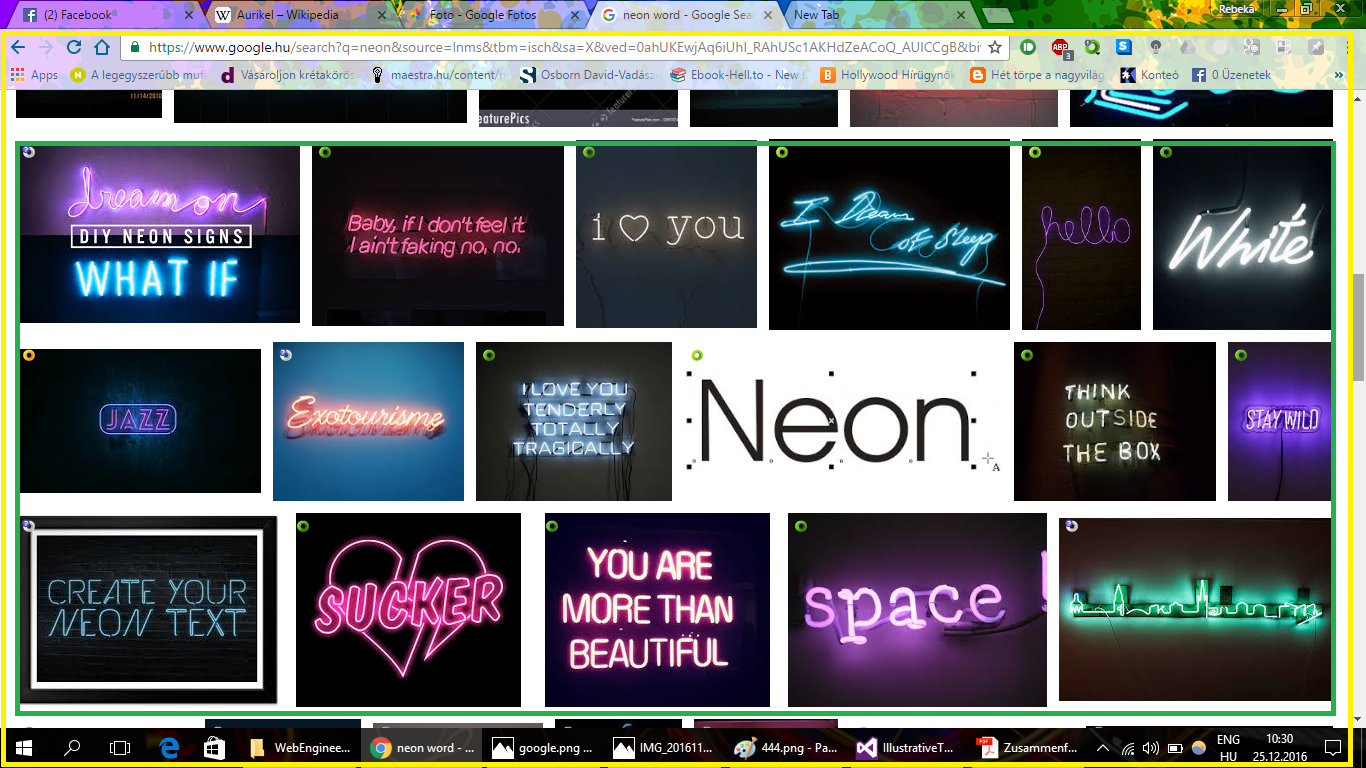
\includegraphics[width=\textwidth]{neonBorderRegion}
			\label{fig:res:neon}
		\end{subfigure}
		\begin{subfigure}[b]{0.45\columnwidth}
			\centering
			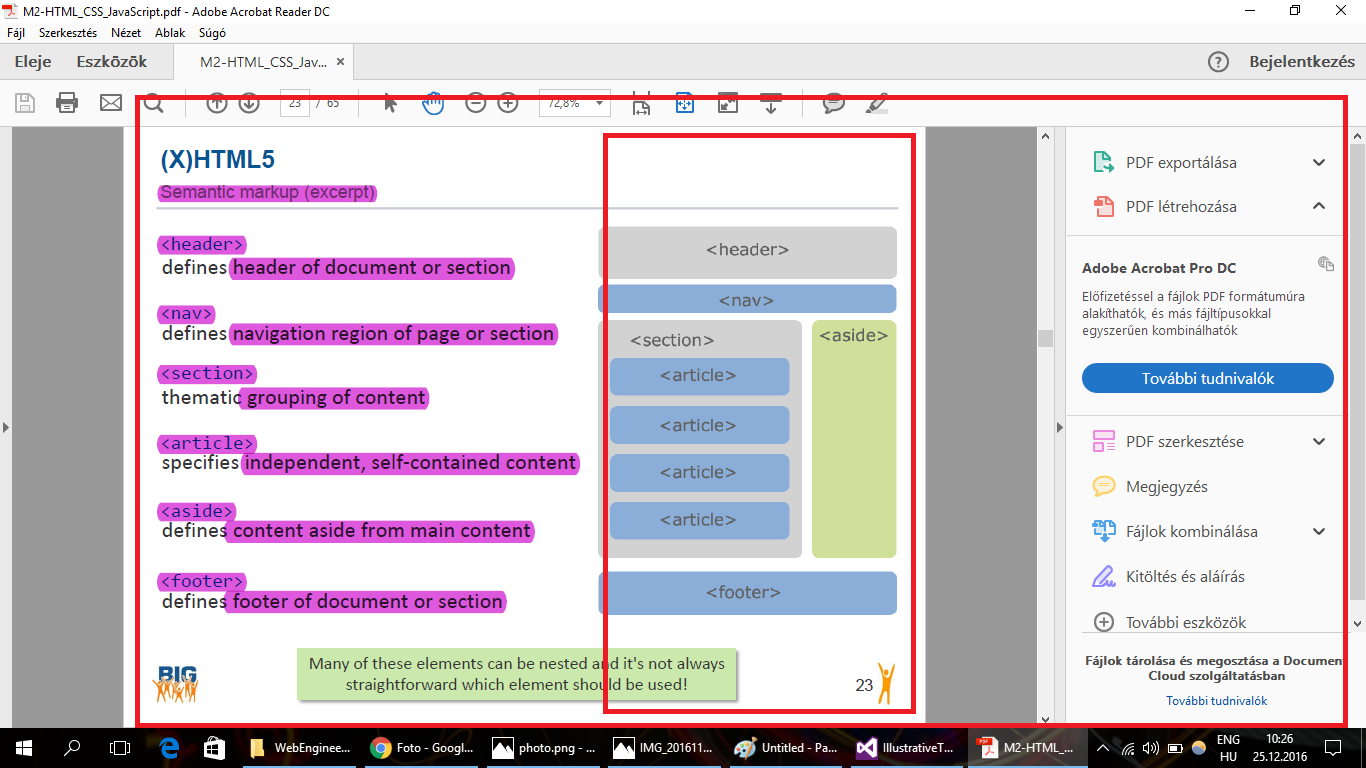
\includegraphics[width=\textwidth]{pdfBorderRegion}
			\label{fig:res:pdf}
		\end{subfigure}
		\caption{The cropping points according to the border area 10\% (yellow) and 40\% (green).}
	 % \label has to be placed AFTER \caption (or \subcaption) to produce correct cross-references.
	\end{figure} 
	Starting from the histograms of the border area, the central area and the slices between them are sequentially compared, the value of their correlation is crucial for assigning them to one or another part of the image.
	If the correlation between the central area and the slice is set for too high, it means their correlation value has to be small (1), some content elements near the border can be eliminated, at low correlation (2.5) however some UI widgets can be labeled as important content. \par
	\begin{figure}[H]
		\centering
		\begin{subfigure}[b]{0.45\columnwidth}
			\centering
			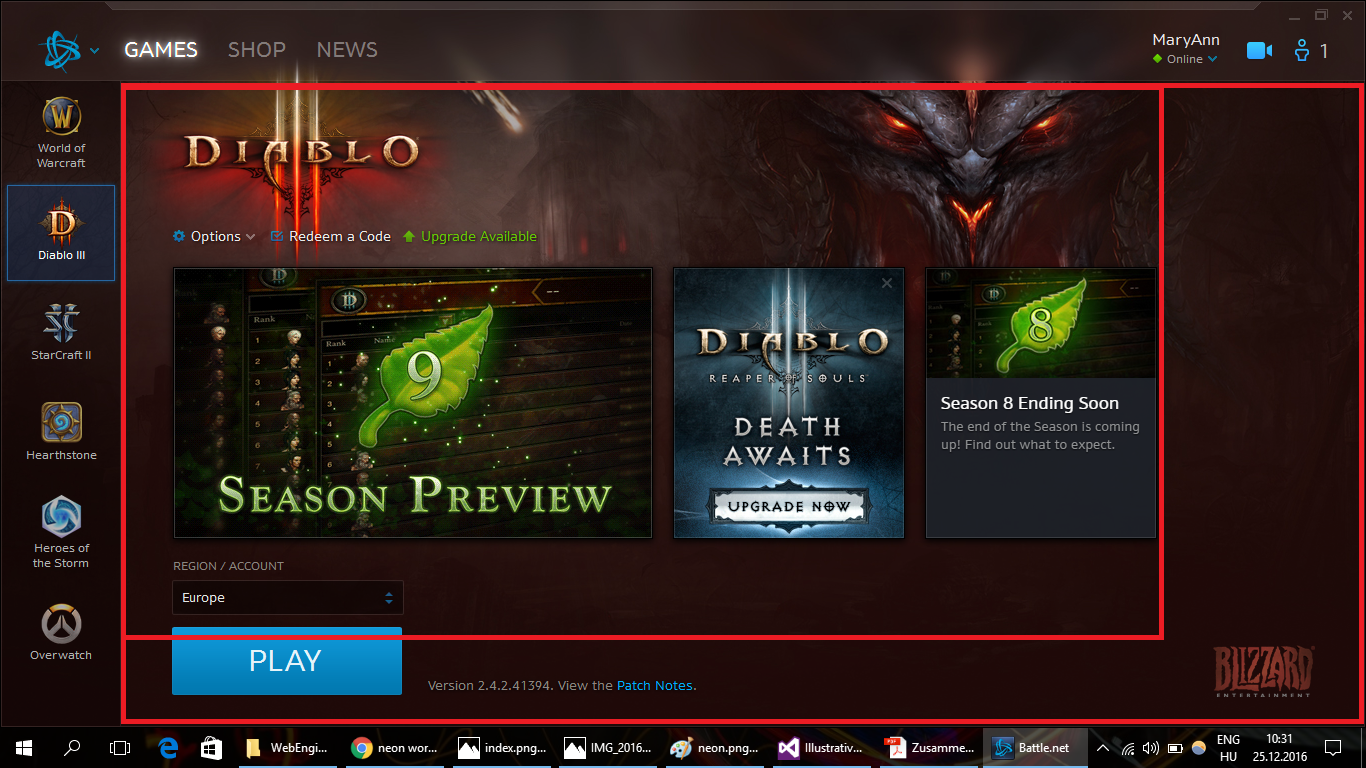
\includegraphics[width=\textwidth]{diabloCorr}
			\label{fig:res:corr1}
		\end{subfigure}
		\begin{subfigure}[b]{0.45\columnwidth}
			\centering
			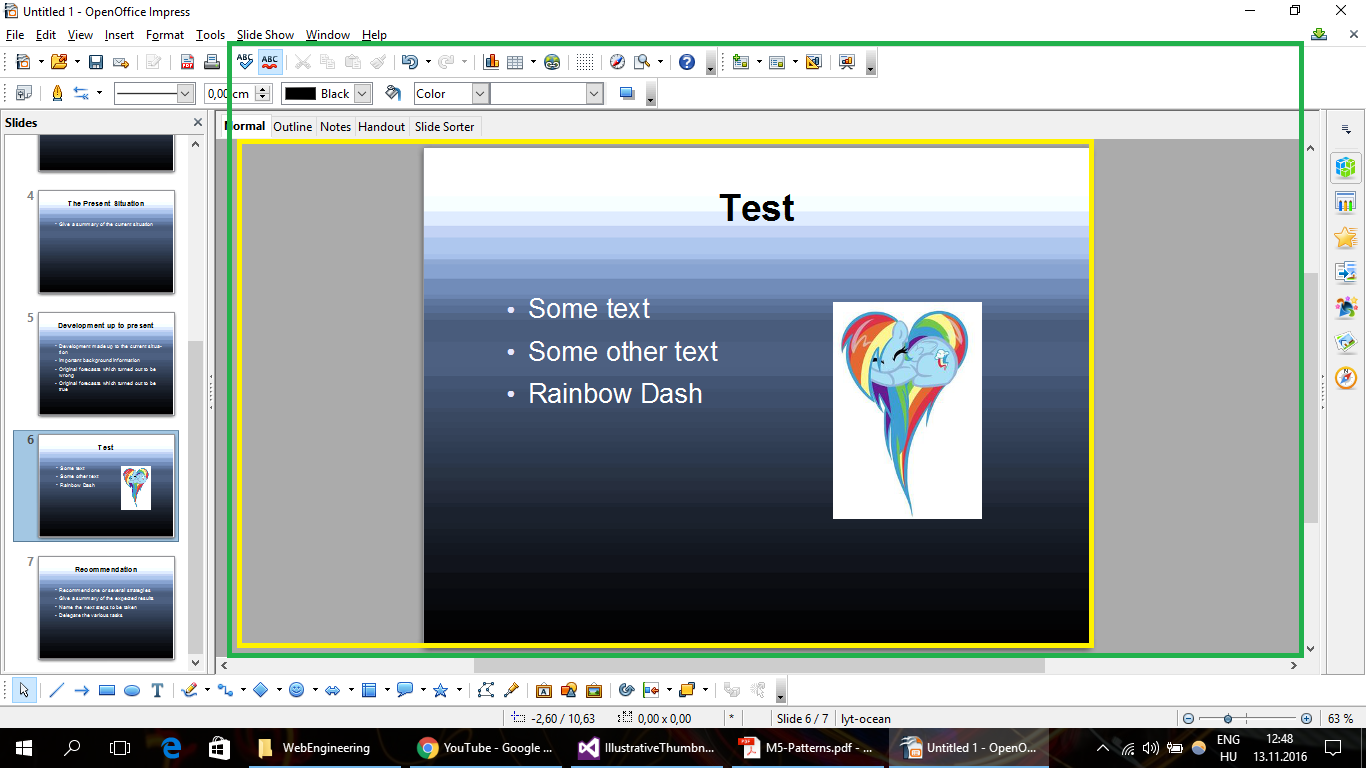
\includegraphics[width=\textwidth]{pptCorr}
			\label{fig:res:corr2}
		\end{subfigure}
		\caption{The cropping points according to the correlation 1 (yellow) and 2.5 (green).}
		 % \label has to be placed AFTER \caption (or \subcaption) to produce correct cross-references.
	\end{figure} 
	The thickness of the slices influences how refined throughout the algorithm is when searching through the border area.
	If the slices are really slim (5\% of the image size) the performance slightly decreases, but in exchange it is able to find a really close cropping point, i.e. where the UI and the content actually meets.\par
	\begin{figure}[H]
		\centering
		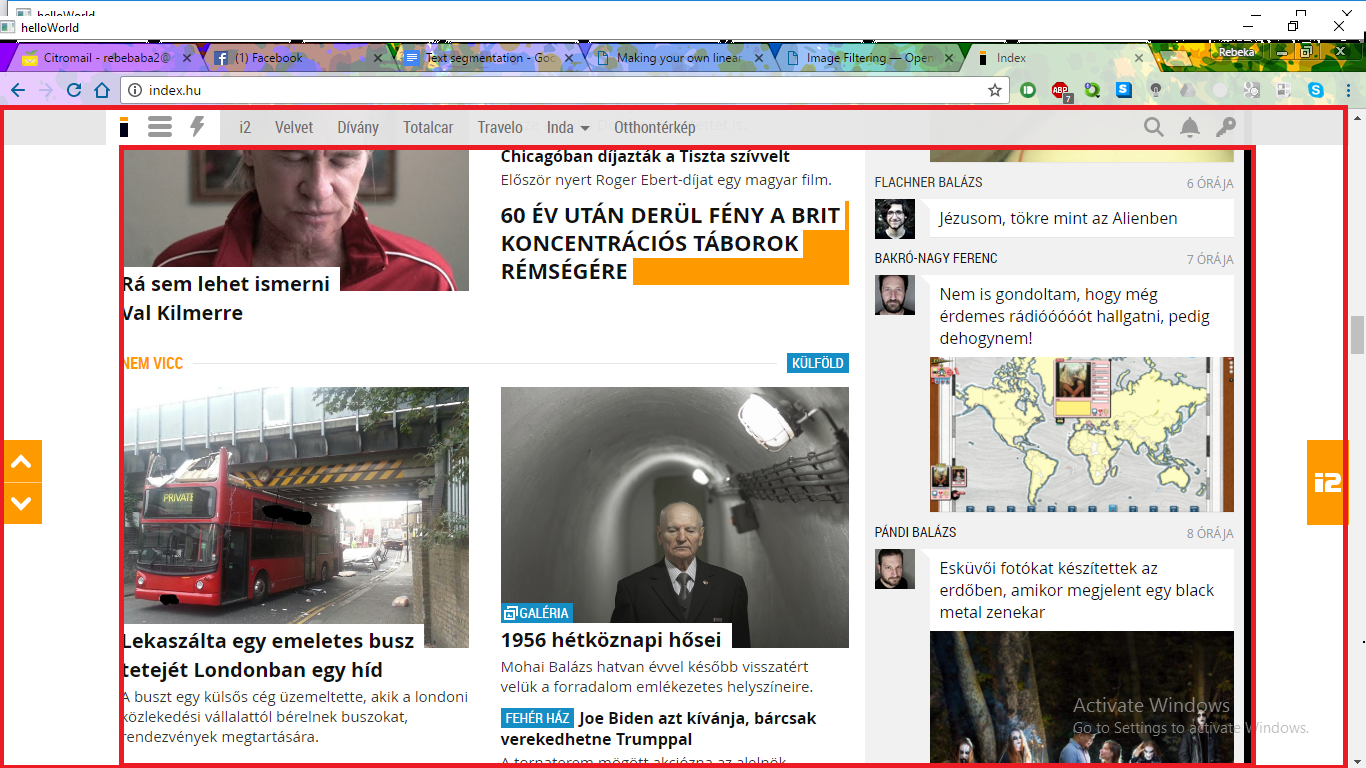
\includegraphics[width=0.5\textwidth]{indexSteps}
		\caption{The cropping points according to the thickness of the slices 12\% (yellow) and 5\% (green)}
		\label{fig:res:steps}
	\end{figure}
	\section{Text detection}
	Because of the Laplacian operator the silhouettes of the letters are highlighted, and a bright color is assigned to them. 
	If these silhouettes are already blurred on the grayscale image, the color of the letters and their area is slightly modified. 
	With the implementation of a threshold range a minimal pixel color value is defined that is in place to have the pixel labeled as possible text.
	If this parameter is small (50) any bright area can be classified as text, even if the given region is only neighboring a word.
	But if it is set to a high value (200), only the core of a word will reach it, so no region will actually contour its related word's shape.
	Bright blue contours the related area, the darker color however shows the regions classified as actual word.\par
	\begin{figure}[H]
		\includegraphics[width=.3\textwidth]{444}\hfill
		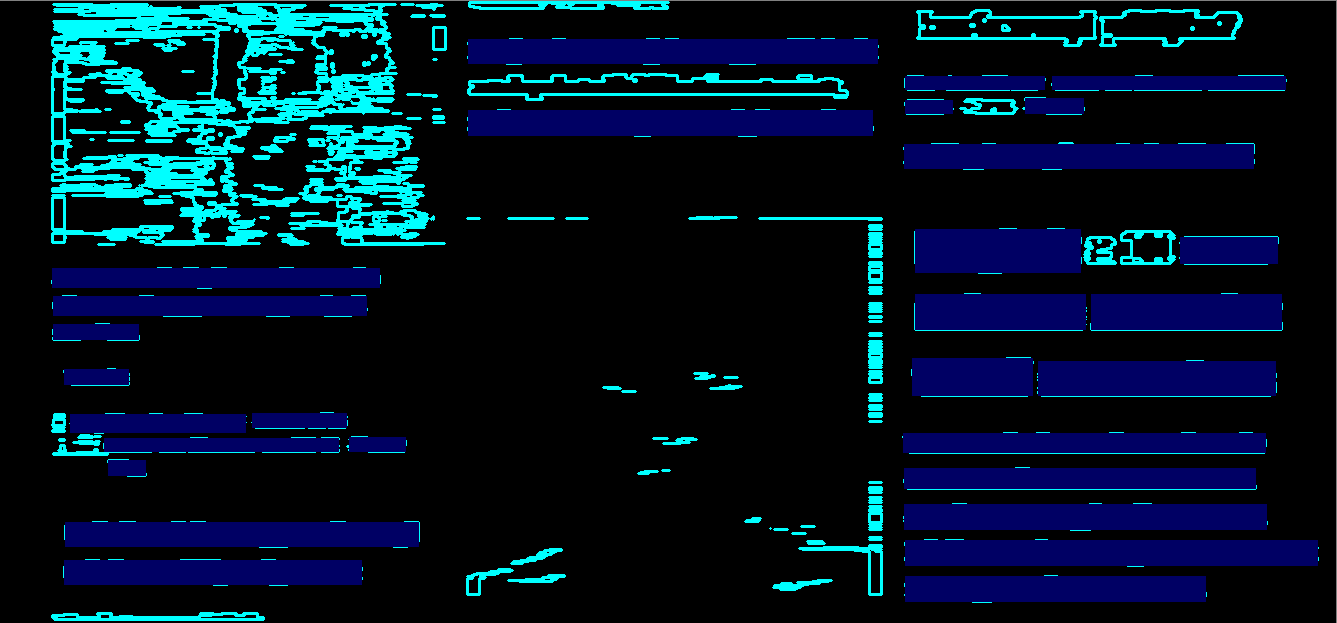
\includegraphics[width=.3\textwidth]{444String50}\hfill
		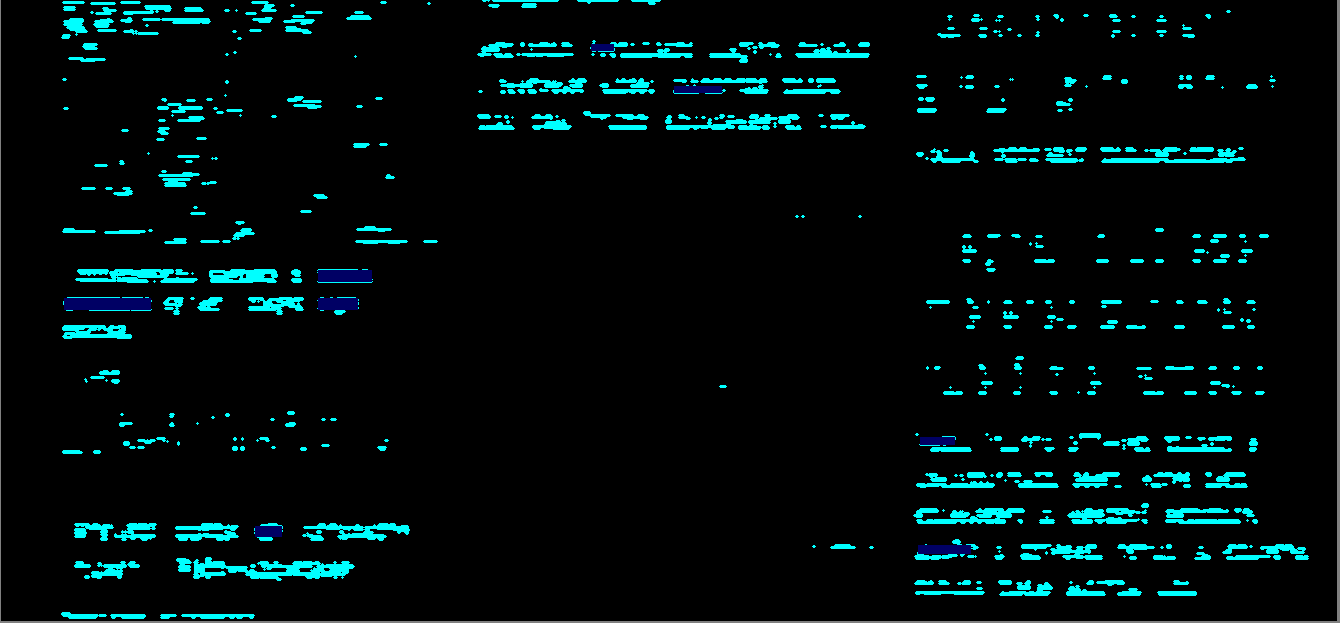
\includegraphics[width=.3\textwidth]{444String200}
		\caption{The related areas according to the brightness threshold value 50 and 200. }
	\end{figure} 
	The properties of a possible word are  in the \texttt{config} file also customizable.
	The set of possible words needs to be sorted first, depending on how likely they are potential words when considering their size.
	The parameters for minimum height and width need to be chosen carefully, since if they are too big (width is set to 100, font size of 12pt, more than 6 letters or height to 20, font size of 14pt), almost every word will get excluded from the list.
	\begin{figure}[H]
		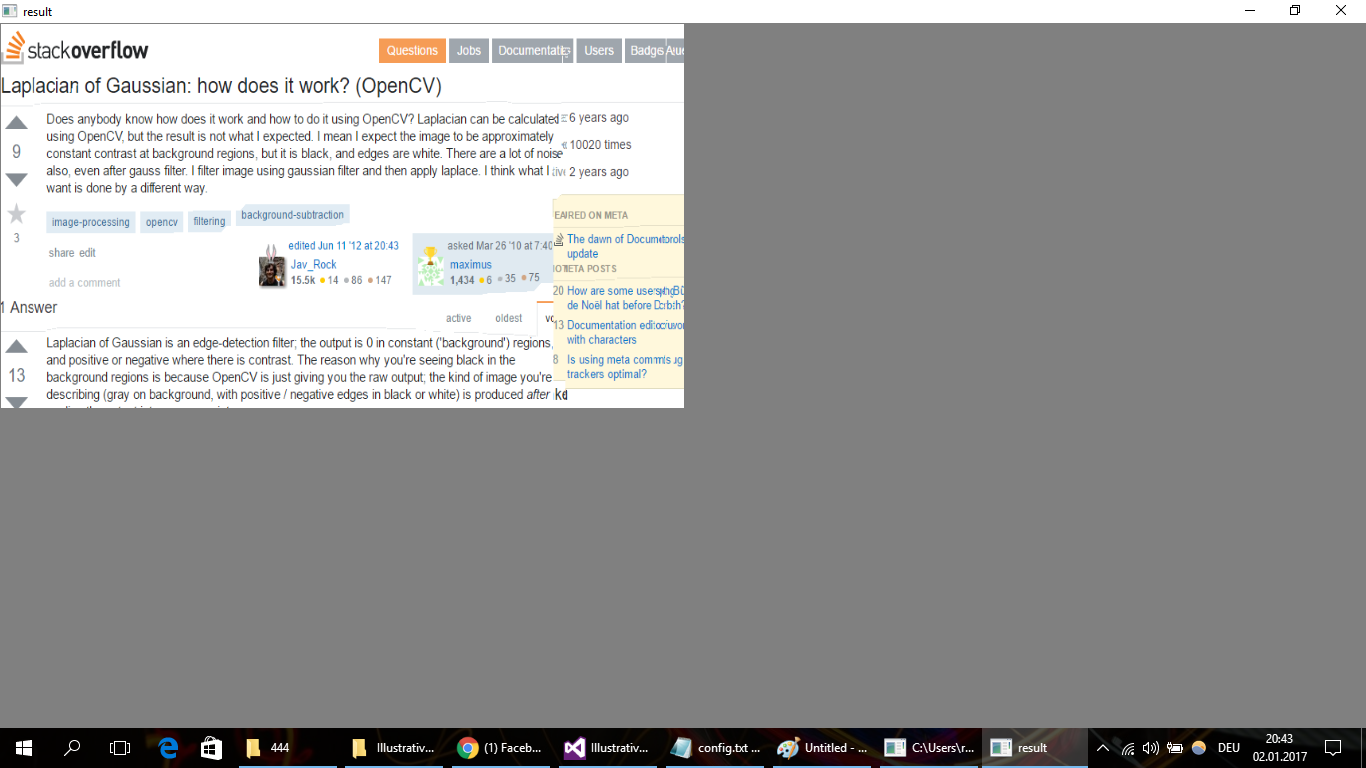
\includegraphics[width=.3\textwidth]{stackOverflow}\hfill
		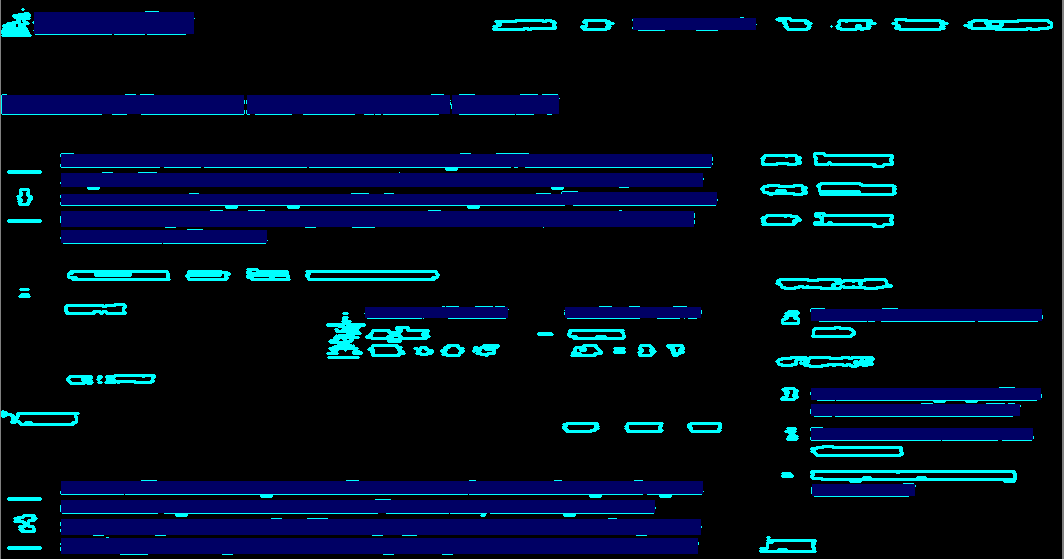
\includegraphics[width=.3\textwidth]{stackOverflowWidth100}\hfill
		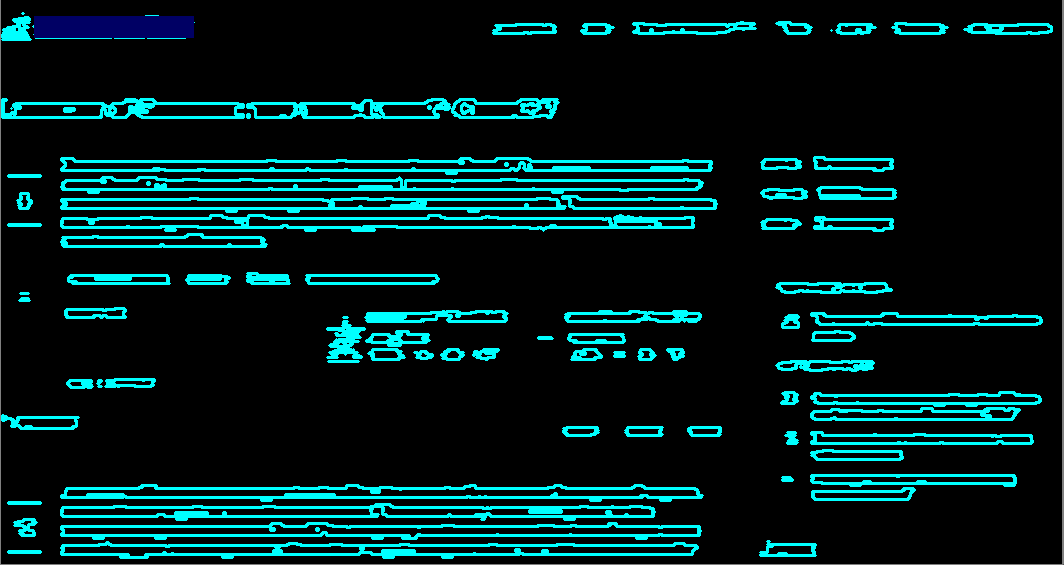
\includegraphics[width=.3\textwidth]{stackOverflowHeight20}
		\caption{The actual words according to the minimal width 100 and minimal height 20. }
	\end{figure}  
	From the set of the possible words the average word size is calculated, but after then it is still further customizable how much the words are allowed to vary from this value.
	For example if the allowed difference is set to 80\% of the original size the smaller words can easily get sorted out, while at 20\% they also manage to stay in the possible words set.\par 
	\begin{figure}[H]
		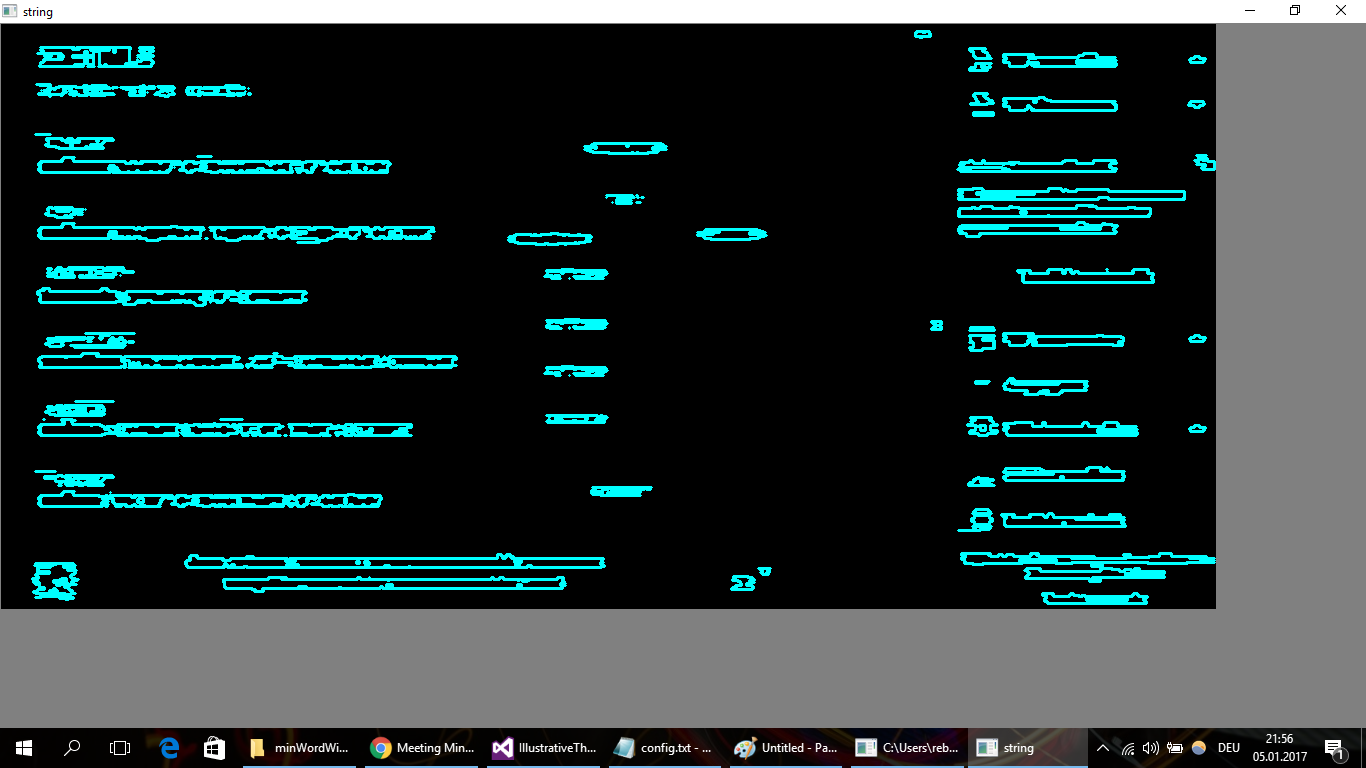
\includegraphics[width=.3\textwidth]{pdf2}\hfill
		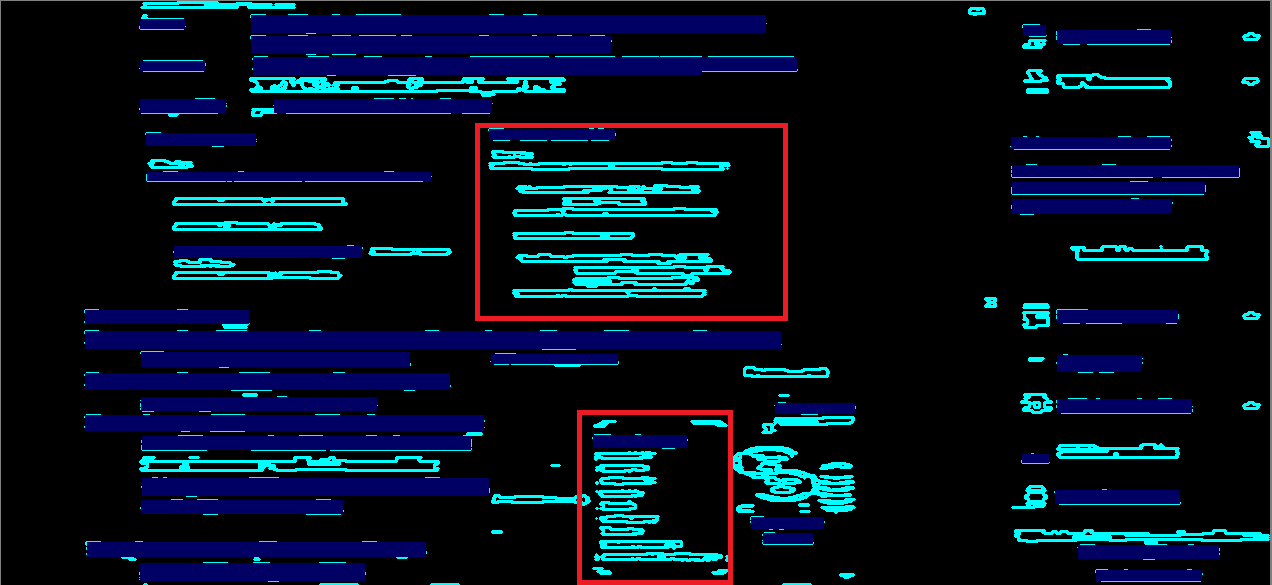
\includegraphics[width=.3\textwidth]{pdf2height80}\hfill
		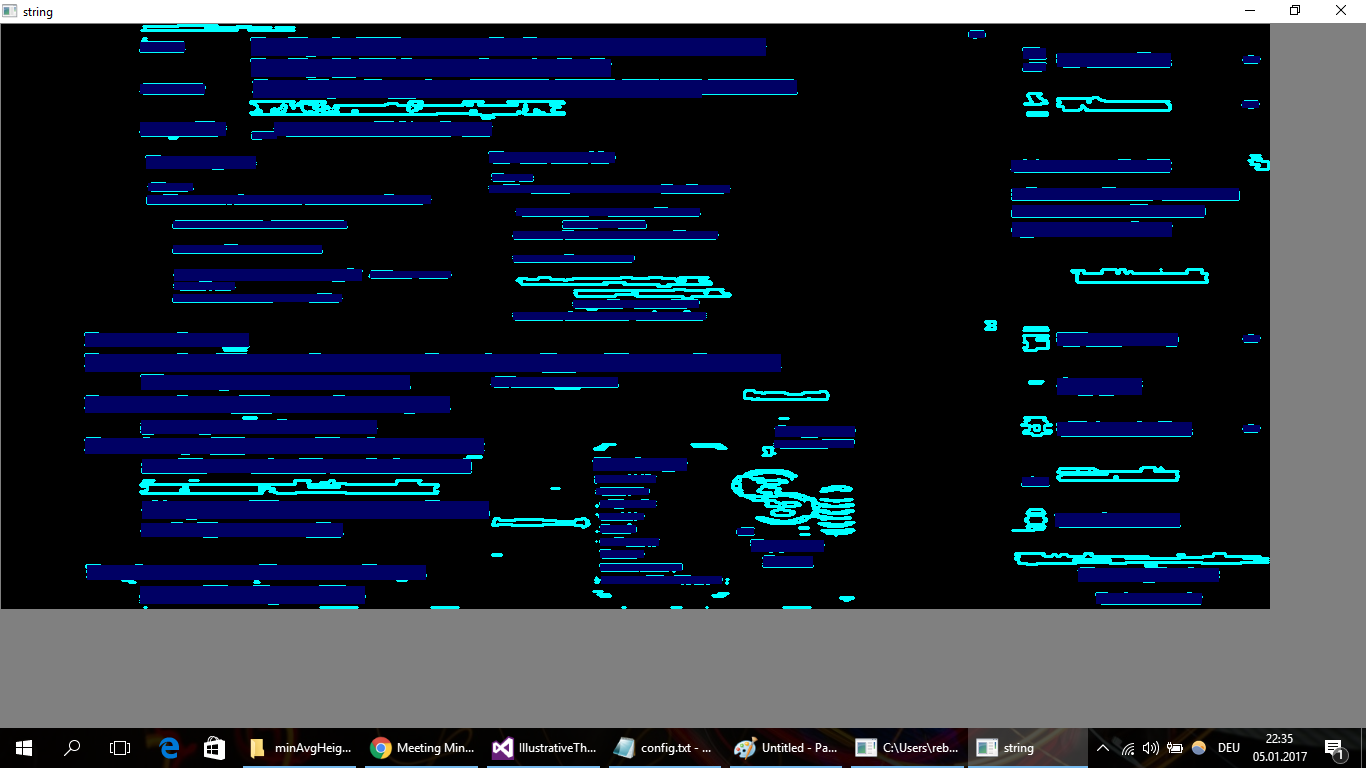
\includegraphics[width=.3\textwidth]{pdf2height20}
		\caption{The actual words according to the maximal allowed difference 80\% and 20\% from the average.  }
	\end{figure}  
	With the inversion of the algorithm, setting the weight of the words for negative, the behavior of the application can be changed.
	For experimental investigation the text areas were set non-salient, so only images and no words are saved. 
	When really small thumbnails are required, it  is advisable to save and present the image data instead of texts, since they would be illegible due to their minuscule size.  
	The experimental results are presented below.
	\begin{figure}[H]		
		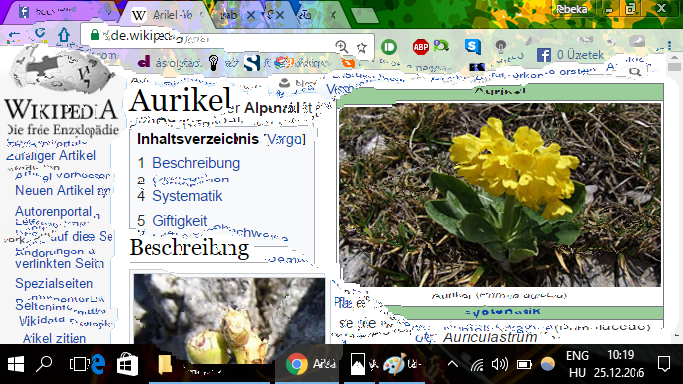
\includegraphics[width=.3\textwidth]{wikipedia}\hfill
		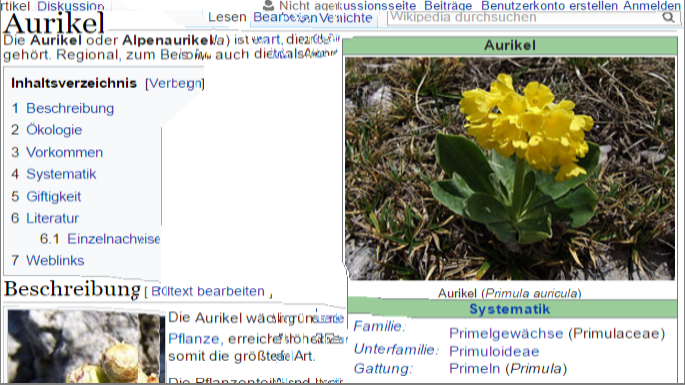
\includegraphics[width=.3\textwidth]{wikiresult}\hfill
		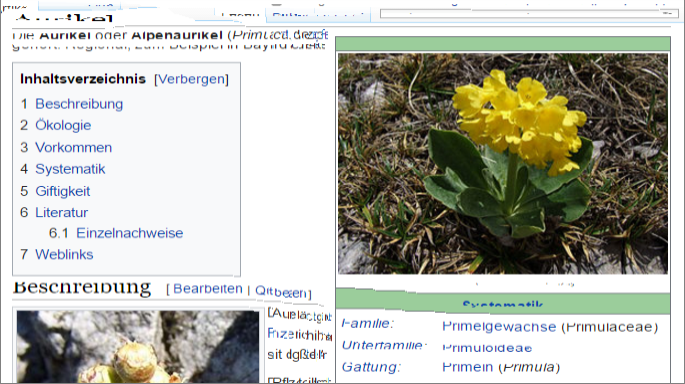
\includegraphics[width=.3\textwidth]{wikiResultNoText}
	
		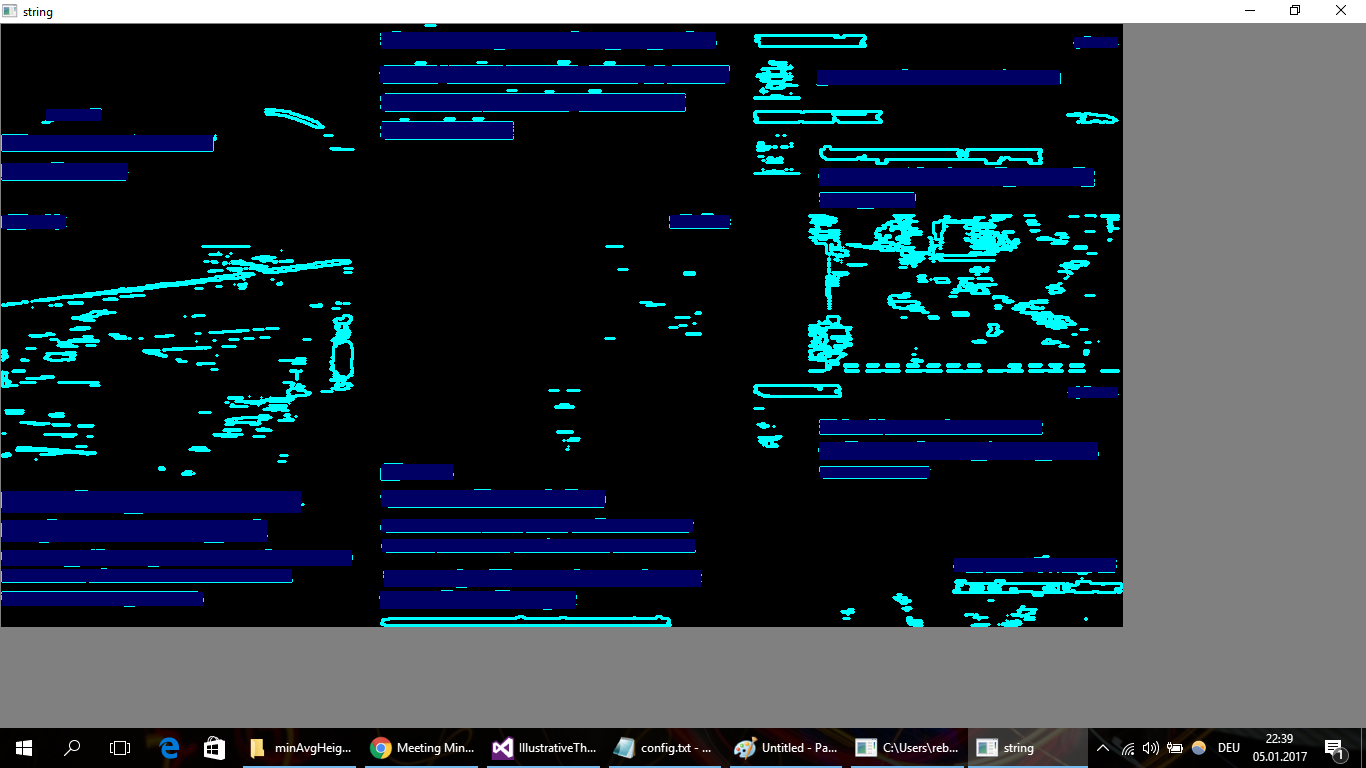
\includegraphics[width=.3\textwidth]{index}\hfill
		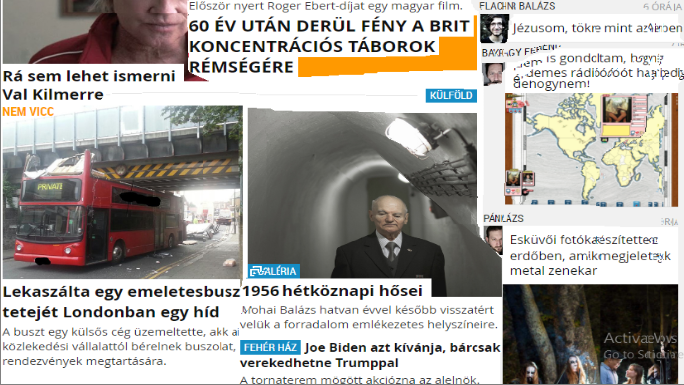
\includegraphics[width=.3\textwidth]{indexresult}\hfill
		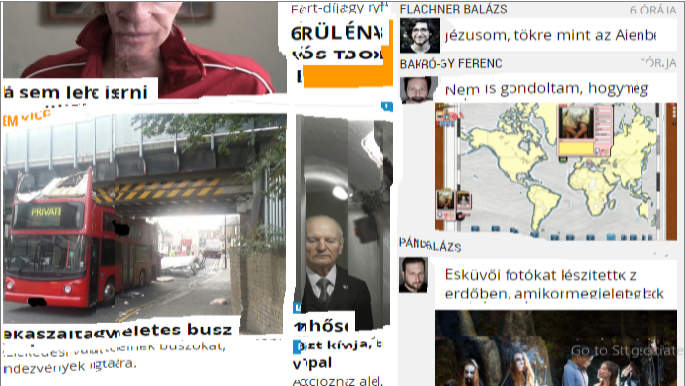
\includegraphics[width=.3\textwidth]{indexResultNoText}
	
		\caption{Different text weighting: high weights (middle) and low weights (right).  }
	\end{figure} 
	\section{Re-sampling threshold}
	\label{res:resampling}
	The re-sampling threshold determines when the application switches from seam carving to usual re-sampling. 
	If the value is small (0.1, 10\% of the average importance of the most important seam on the original image) only a few seam carving loops are performed, and the application behaves similar to a common down-sampling algorithm.
	The performance is positively affected by fewer seam carving loops, but it also loses its advantage against simple re-sampling methods, with the important areas being no longer easily recognizable.
	When the threshold is set, however, to a bigger value (0.4, 40\% of the average importance of the most important seam on the original image), the application switches at the very end of the process.
	In this case the application works noticeably slower and additionally in causes more artifacts than usual re-sampling.
	On Figure~\ref{fig:res} the red lines indicate the edges, where the side-effects of elimination are obvious.
	\begin{figure}[H]
		\centering
		\begin{subfigure}[b]{0.45\columnwidth}
			\centering
			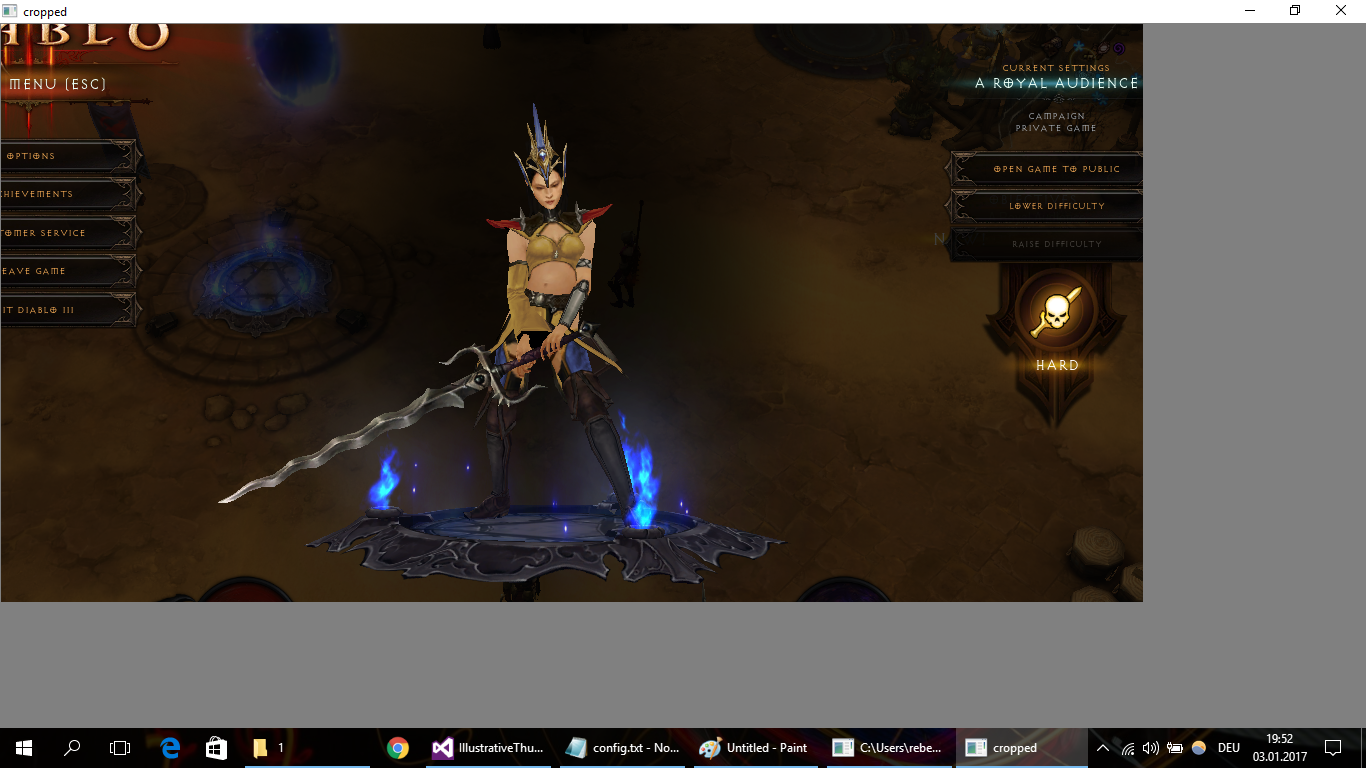
\includegraphics[width=\textwidth]{resamplingTh/game1}
			\label{fig:res:th1}
		\end{subfigure}
		\begin{subfigure}[b]{0.45\columnwidth}
			\centering
			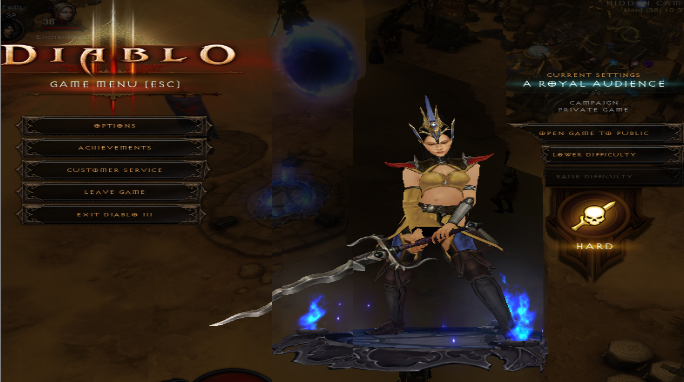
\includegraphics[width=\textwidth]{resamplingTh/game4}
			\label{fig:res:th2}
		\end{subfigure}
		\caption{The results according to the re-sampling threshold 0.1 and 0.4.}
		\label{fig:res}
		% \label has to be placed AFTER \caption (or \subcaption) to produce correct cross-references.
	\end{figure}  
	\section{Comparison to Adobe Photoshop} 
	To compare the algorithm to an already existing tool the content-aware resize feature of Adobe Photoshop CS 5~\cite{photoshop} was used.
	\begin{figure}[H]
		\includegraphics[width=.3\textwidth]{photoshop/org/444}\hfill
		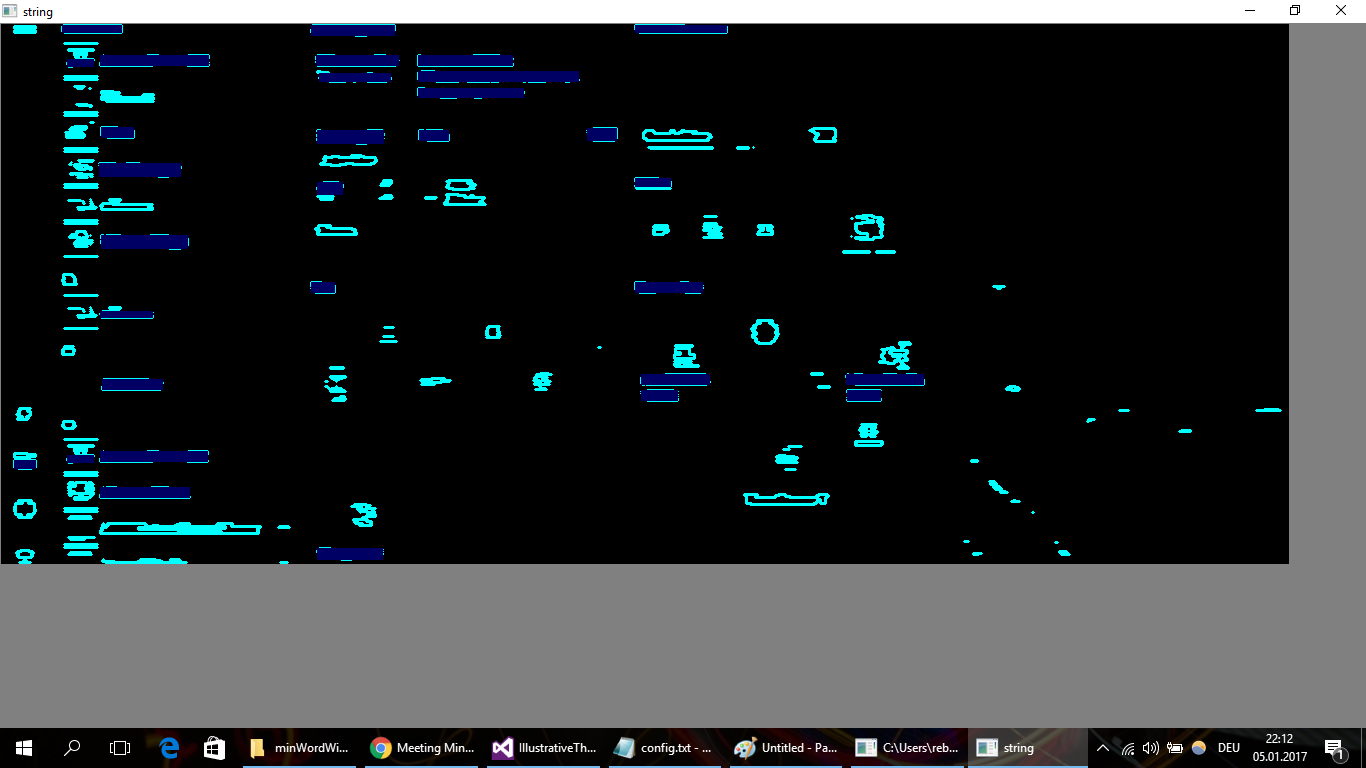
\includegraphics[width=.3\textwidth]{photoshop/org/desktop}\hfill
		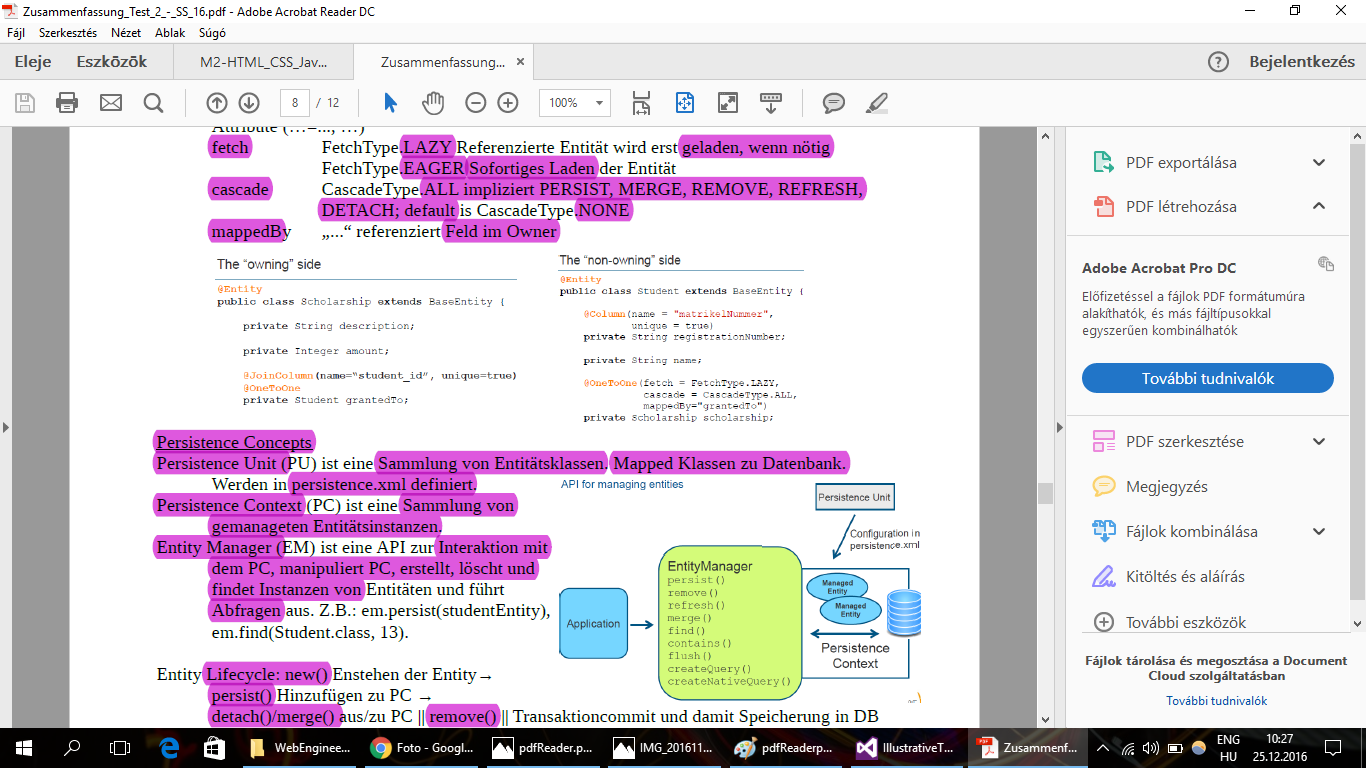
\includegraphics[width=.3\textwidth]{photoshop/org/pdfReader2}
		\caption{Source images used for testing}
	\end{figure}
	There are two test scenarios; the first takes the same source to the illustrative thumbnail creator algorithm.
	The input image in the second case is however the cropped source image produced by this application after the elimination of the UI elements.
	In the first test it is investigated how seam carving invented for usual photos works on screenshots.
	\begin{figure}[H]
		\includegraphics[width=.3\textwidth]{photoshop/444}\hfill
		\includegraphics[width=.3\textwidth]{photoshop/desktop}\hfill
		\includegraphics[width=.3\textwidth]{photoshop/pdf1}
		\caption{Photoshop results of the first scenario.}
	\end{figure}
	Comparing  the images to outputs of the thumbnail algorithm, it is striking how much smaller and less readable the words appear.
	Because this project applies not only seam carving but also heuristics to cut off the border region, to compare the actual seam carving algorithms, Photoshop  needs the same input as this application has, when it starts the seam calculation.
	The second test scenario is in place for this reason.
	\begin{figure}[H]
		\includegraphics[width=.3\textwidth]{photoshop/444cropped}\hfill
		\includegraphics[width=.3\textwidth]{photoshop/desktopcropped}\hfill
		\includegraphics[width=.3\textwidth]{photoshop/pdf1cropped}
		\caption{Photoshop results of the second scenario.}
	\end{figure}
	The quality of the  output definitely improves: face is recognizable, text is easier to read, icons are preserved, since an already smaller image needs to shrunk to the same size as before.
	The main difference between the two methods seems to lay on the weighting of the content.
	This approach pays more attention to the text, with image data being easily ignored.
	\begin{figure}[H]
		\includegraphics[width=.3\textwidth]{photoshop/default/444}\hfill
		\includegraphics[width=.3\textwidth]{photoshop/default/desktop}\hfill
		\includegraphics[width=.3\textwidth]{photoshop/default/pdf}
		\caption{Result of the thumbnail algorithm}
	\end{figure}
	Photoshop, however, attempts to sustain the image content.
	Since the thumbnail creator algorithm has a ranking between the elements, holding texts before images, the output is not dubious: even in case of image data loss, the text remains readable, like the snippet of Figure~\ref{fig:comp444} shows.
	The output of Photoshop is rather disorganized, the text and image regions flow into each other, illustrated on Figure~\ref{fig:compDesktop}.
	The images are better recognizable as already illustrated on Figure~\ref{fig:comp444}, but in exchange the words are noticeably more damaged, like the code snippets on Figure~\ref{fig:comppdf}. 
	All results produced by Photoshop are listed in \hyperref[AppB]{Appendix B}. 
	
	\begin{figure}[H]
		\centering		
		\includegraphics[width=\textwidth]{photoshop/compare444}
		\caption{Snippet about the same region of the first test image captured on the output of the Photoshop test scenarios and of the thumbnail creator algorithm }
		\label{fig:comp444}
	\end{figure}
	\begin{figure}[H]
		\centering		
		\includegraphics[width=\textwidth]{photoshop/compareDesktop}
		\caption{Snippet about the same region of the second test image captured on the output of the Photoshop test scenarios and of the thumbnail creator algorithm.}
		\label{fig:compDesktop}
	\end{figure}
	\begin{figure}[H]
		\centering		
		\includegraphics[width=0.5\textwidth]{photoshop/comparePdf}
		\caption{Snippet about the same region of the third test image captured on the output of the Photoshop test scenarios and of the thumbnail creator algorithm.}
		\label{fig:comppdf}
	\end{figure}
	
	\section{Natural Images}
	The algorithm is meant for the creation of expressive thumbnails but nor for down-sampling natural images.
	The importance map calculation is customized for the requirements of a screenshot, not of a common photograph.
	There are two aspects, where the thumbnail algorithm fails, and it is not able to provide results having the same quality as before.
	The first one is the UI cropping heuristic, as shown in Figure~\ref{fig:nat:face}.
	It is common also on natural images, that the margin area has slightly other color theme than the central region.
	At the margin normally the background is shown, whereas the focus objects of the picture are placed at the middle of the scene.
	Because of that it is possible, since the UI cropping algorithm examines only the color histograms of both areas, that it assumes, that at the margin UI widget are found, and some border parts get eliminated.
	\begin{figure}[H]
		\centering
		\begin{subfigure}[b]{0.45\columnwidth}
			\centering
			\includegraphics[width=\textwidth]{img/face}
		\end{subfigure}
		\begin{subfigure}[b]{0.45\columnwidth}
			\centering
			\includegraphics[width=\textwidth]{img/resFace}
		\end{subfigure}
		\caption{The UI cropping heuristic eliminates two persons on the right side.}
		\label{fig:nat:face}
		% \label has to be placed AFTER \caption (or \subcaption) to produce correct cross-references.
	\end{figure}  
	Other drawbacks of the thumbnail algorithm on natural images are the artifacts caused by seam carving.
	There are two problems, why the algorithm is not able to work on photographs from the real word as smooth as on screenshot images.
	The first one is the importance map calculation, which is as mentioned above is customized for computer screens and not for natural images.
	So the seam carving method has later no information about which object should be handled special, as it has about text data earlier.
	The second one is, that there are no post-processing step after the seam elimination.	
	The transition between the objects on computer screens is not so smooth like it is on natural images.
	Sharp edges and strong intensity changes on screenshots are usual, so even after seam carving the possibly artifacts caused by pixel elimination are not so outstanding, because it is usual also on the original image.
	By processing natural images, in order to they look further natural it would be necessary however, to smooth the edges left behind by the eliminated pixel paths.
	Since this step is not implemented, the hints of the image processing are obvious on Figure~\ref{fig:nat:food} and on Figure~\ref{fig:nat:fire}.  
	\begin{figure}[h]
		\centering
		\begin{subfigure}[b]{0.45\columnwidth}
			\centering
			\includegraphics[width=\textwidth]{img/food}
		\end{subfigure}
		\begin{subfigure}[b]{0.45\columnwidth}
			\centering
			\includegraphics[width=\textwidth]{img/resfood}
		\end{subfigure}
		\caption{There is a horizontal line in the middle, where probably several seems were eliminated.}
		\label{fig:nat:food}
		% \label has to be placed AFTER \caption (or \subcaption) to produce correct cross-references.
	\end{figure}  
	\begin{figure}[h]
		\centering
		\begin{subfigure}[b]{0.45\columnwidth}
			\centering
			\includegraphics[width=\textwidth]{img/firework}
		\end{subfigure}
		\begin{subfigure}[b]{0.45\columnwidth}
			\centering
			\includegraphics[width=\textwidth]{img/resFirework}
		\end{subfigure}
		\caption{There are several artifact to see on the body of the fireworks.}
		\label{fig:nat:fire}
		% \label has to be placed AFTER \caption (or \subcaption) to produce correct cross-references.
	\end{figure}    
	
	
	\section{Performance Evaluation}
	The tests were performed on Windows 10 with CPU Intel i3-2310, 2.1GHZ and 2 Cores, using Grafic card AMD Radeon HD 7400M.
	During the tests some performance issues occurred, the application occasionally needed up to 3.5 minutes performance time, however remaining in a one-minute termination average.\par 
	The performance bottleneck is caused by seam calculation.
	Every time when a seam is eliminated, the whole saliency map is recalculated.
	Having a new saliency map the possible seam paths also need to get redetermined.
	If the UI cropping algorithm is not able to cut a bigger area or the re-sampling threshold is reached later, several seam carving loops are performed. 
	Therefore, screenshots with bigger and clearly defined UI areas have shorter run time, whereas inputs like images of gallery applications and of computer games take longer. 
	
	\chapter{Future Work}
	\label{futureWork}
	This application, according to the chapter above, is effective at creating illustrative thumbnails, but there are certain implementations to extend its scope. 
	There are two main improvement areas to investigate: performance and software methodology.
	Although the current application provides reasonable results, as described in the preceding chapters, there are several approaches, to make the present method even more robust and easier to use.
	The most important directions for development will be discussed in the following section.
	
	\section{Performance improvement} 
	The core task of a seam carving algorithm is the evaluation of the saliency map.
	Optimally, every pixel and every possible path are needed to be examined in order to find the most favorable path.
	Depending on the size of the input, visiting and checking all pixels individually can take a long time.
	This process can be get, however, easily parallelized.
	In 2007, Nvidia released a parallel computing platform, called CUDA~\cite{Cook:2012:CPD:2430671}, which exploits the computing performance of the GPU.
	The CUDA system can be simply integrated into the current application, since it is developed for programming languages C, C++ and Fortran, that includes the C++ used in this project.
	In addition, seam carving is already implemented on the system by Duarte et al.~\cite{duarte2012accelerating}.
	
	\section{Methodology improvement}
	An essential challenge in seam carving is the construction of the saliency map and the calculation of the seams. 
	The methods implemented in the current project are able to handle most standard cases, on the other hand, with some improvements it has the potential to became more robust and usable in even more special cases.\par 
	There are several approaches that besides the low level pixel data examination, aim to find also semantically meaningful objects in the input.
	They are building on the observation, that some objects, for example faces, even if their coloring is not special, are very important for human viewers.
	The perceptual seam carving algorithm from Hwang et al.~\cite{hwang2008content}, based on the Human Attention Model, calculates not only the color changes but also the occurrence of facial information, so the output in the case of Figure~\ref{fig:face} would change.
	\begin{figure}[H]
		\centering
		\begin{subfigure}[b]{0.45\columnwidth}
			\centering
			\includegraphics[width=\textwidth]{photoshop/org/444}
			\label{fig:res:th1}
		\end{subfigure}
		\begin{subfigure}[b]{0.45\columnwidth}
			\centering
			\includegraphics[width=\textwidth]{photoshop/default/444}
			\label{fig:res:th2}
		\end{subfigure}
		\caption{The current algorithm destroys the facial information.}
		\label{fig:face}
		% \label has to be placed AFTER \caption (or \subcaption) to produce correct cross-references.
	\end{figure}  	
	It includes an already implemented feature of OpenCV, with which the application is able to generate a face map.
	The energy function, which calculates the pixel values in the saliency map, is then weighted with the data from the face map, so an even more detailed saliency map is constructed.\par 
	Furthermore, apart from the face information, Domingues et al.~\cite{domingues2010stream} also use gradient magnitude, Canny edge detection and Hugh line detection to make the saliency map as meaningful as possible. 
	It thoroughly examines both the semantic and the low level pixel data.
	There is, however, another method to evaluate the pixel information in an even more profound manner.
	Putting the information into a context makes the measurements more accurate, than the current application, because it controls for information extremities.
	Consequently, no pixel will appear more important - or unimportant - than it really is.
	Guo et al.~\cite{guo2015nif} obtain this with the calculation of a so-called neighborhood inhomogeneity factor, which denotes the amount of inhomogeneous neighbors of every pixel. 
	This approach helps to find the important areas inside an object, where a simple line detection algorithm fails i.e. indicate no salient regions.
	The saliency map where, according to the algorithm, also the inside of the object is filled, is showed on Figure~\ref{fig:nif}.
	\begin{figure}[H]
		\centering		
		\includegraphics[width=0.5\textwidth]{NIF}
		\caption{The source image and the saliency map of the NIF algorithm ~\cite{guo2015nif} }
		\label{fig:nif}
	\end{figure}
	To find the coherent areas that later can be defined as objects, the use of a mean shift algorithm, as Liu et al.~\cite{liu2006region} does, would be effective. 
	Furthermore, this algorithm makes the saliency calculation scale invariant, and decreases the chance of finding misleadingly high important edges.
	The resulting saliency map is showed in Figure~\ref{fig:kmean}.\par
	\begin{figure}[H]
		\centering		
		\includegraphics[width=0.5\textwidth]{kMeans}
		\caption{The source image and the saliency map of the mean shift algorithm ~\cite{liu2006region} }
		\label{fig:kmean}
	\end{figure} 
	When the saliency map is final, the next step is to calculate the seams.
	In this project seams are defined as paths with the width of one pixel.
	On the other hand, moderation of this rule can provide better results with less artifacts and also increases of performance, as obtained by Domingues et al.~\cite{domingues2010stream}.
	This approach tries to find streams, seams wider than only one pixel, to eliminate bigger areas of the picture at once.
	Even if the cheapest seams are not neighboring, for the cost of eliminating a slightly greater salient region, the number of needed loops per image can be decreased.
	The most important precondition is that the stream is not allowed to cross any salient line or region, for example faces, so the relative saliency value still needs to stay low. \par
	In order to eliminate the possible artifacts caused by cutting of seams and streams an algorithm presented by  Sun et al~\cite{sun2005image} offers help.
	This approach is also based on saliency calculation.
	If there is a big area, which needs to be filled up, it investigates the saliency map and the texture of the neighboring regions.
	The most salient points are then labeled as anchor points; the actual task is to find a connection between these anchors and to color the background, as shown on Figure~\ref{fig:structProp}.
	\begin{figure}[H]
		\centering		
		\includegraphics[width=0.5\textwidth]{strctProp}
		\caption{The structure propagation algorithm, where $\Omega$ denotes the unknown regions and $p_{i}$ the anchor points ~\cite{sun2005image}} 
		\label{fig:structProp}
	\end{figure}
	In case of seam carving the goal is not to recreate the eliminated areas but with the above algorithm it is possible to make transition areas smoother.
	If a stream is taken, a narrow, only a few pixel wide path can be left behind, to let the algorithm work.
	In the case of seams however the neighboring edges can be modified according to the filling method, taking some wider area around the seam as reference.\par 
	A further possibility to make the current algorithm faster and able to deal with the artifacts better is presented by Dong et al.~\cite{dong2009optimized}.
	This method has to slightly modify the pipeline of the project, since it employs usual re-sampling in the seam carving phase already.
	It classifies every pixel on the input image as foreground, very salient, related objects, and background, less salient, probably split up parts of the image.
	The seam carving method is applied only on the foreground data, the non-salient regions are processed with simple re-sampling. 
	With this approach the properties of the background have no influence on the actual sequence of seam.
	The calculation needs to take only the saliency values of the important foreground objects into account, therefore the resulting path will be more accurate and consist the most important regions of the picture.
	Furthermore, in this case a seam is shorter than it would be when it was be applied to the whole input, as it is only calculated for certain foreground objects, causing significantly smaller and less noticeable artifacts.
	As an additional favorable side effect, also the performance increases due to the decreased amount of areas to be considered for the seam calculation.\par
	All improvements suggested in this section are developed for natural images.
	In the case of their use, these methods need some modification to function also by thumbnails properly.
	When these approaches are implemented, the fact needs to be considered, that they are tested on natural images, and they can possibly have different behavior while using them for thumbnail creation.     
	
	\chapter{Conclusion}
	To make thumbnails more illustrative and applicable even on small screens, a thumbnail creating method using seam carving was presented in this paper.
	In order to obtain the most informative results possible the saliency calculation was adjusted to the special requirements of a screenshot.
	In addition to seam calculation, the presence of UI elements on a computer screen were also taken into account.
	As a combined results of the customized seam carving algorithm and its extensions with other helpful methods such as UI part elimination, text recognition and common re-sampling, the created thumbnails are more illustrative than their usual relatives, since their information content is better recognizable and the text regions are easier to read. 
	
	% Remove following line for the final thesis.
	%%% intro.tex
%% Copyright (C) 2014-2016 by Thomas Auzinger <thomas@auzinger.name>
%
% This work may be distributed and/or modified under the
% conditions of the LaTeX Project Public License, either version 1.3
% of this license or (at your option) any later version.
% The latest version of this license is in
%   http://www.latex-project.org/lppl.txt
% and version 1.3 or later is part of all distributions of LaTeX
% version 2005/12/01 or later.
%
% This work has the LPPL maintenance status `maintained'.
%
% The Current Maintainer of this work is Thomas Auzinger.
%
% This work consists of the files vutinfth.dtx and vutinfth.ins
% and the derived file vutinfth.cls.
% This work also consists of the file intro.tex.


\newacronym{ctan}{CTAN}{Comprehensive TeX Archive Network}
\newacronym{faq}{FAQ}{Frequently Asked Questions}
\newacronym{pdf}{PDF}{Portable Document Format}
\newacronym{svn}{SVN}{Subversion}
\newacronym{wysiwyg}{WYSIWYG}{What You See Is What You Get}

\newglossaryentry{texteditor}
{
  name={editor},
  description={A text editor is a type of program used for editing plain text files.}
}

\chapter{Introduction to \LaTeX}

Since \LaTeX\ is widely used in academia and industry, there exists a plethora of freely accessible introductions to the language.
Reading through the guide at \url{https://en.wikibooks.org/wiki/LaTeX} serves as a comprehensive overview for most of the functionality and is highly recommended before starting with a thesis in \LaTeX.

\section{Installation}

A full \LaTeX\ distribution\index{distribution} consists of not only of the binaries that convert the source files to the typeset documents, but also of a wide range of packages and their documentation.
Depending on the operating system, different implementations are available as shown in Table~\ref{tab:distrib}.
\textbf{Due to the large amount of packages that are in everyday use and due to their high interdependence, it is paramount to keep the installed distribution\index{distribution} up to date.}
Otherwise, obscure errors and tedious debugging ensue.

\begin{table}
  \centering
  \begin{tabular}{cccc}
    \toprule
    Distribution & Unix         & Windows      & MacOS        \\
    \midrule
    TeX Live     & \textbf{yes} & yes          & (yes)        \\
    MacTeX       & no           & no           & \textbf{yes} \\
    MikTeX       & no           & \textbf{yes} & no           \\
    \bottomrule
  \end{tabular}
  \caption{\TeX/\LaTeX\ distributions for different operating systems. Recomended choice in \textbf{bold}.}
  \label{tab:distrib} % \label has to be placed AFTER \caption to produce correct cross-references.
\end{table}

\section{Editors}

A multitude of \TeX\ \glspl{texteditor} are available differing in their editing models, their supported operating systems and their feature sets.
A comprehensive overview of \glspl{texteditor} can be found at the Wikipedia page  \url{https://en.wikipedia.org/wiki/Comparison_of_TeX_editors}.
TeXstudio (\url{http://texstudio.sourceforge.net/}) is recommended.
Most editors support the scrolling the typeset preview document to a location in the source document by \verb|Ctrl| clicking the location in the source document.

\section{Compilation}

Modern editors usually provide the compilation programs to generate \gls{pdf} documents and for most \LaTeX\ source files, this is sufficient.
More advanced \LaTeX\ functionality, such as glossaries and bibliographies, needs additional compilation steps, however.
It is also possible that errors in the compilation process invalidate intermediate files and force subsequent compilation runs to fail.
It is advisable to delete intermediate files (\verb|.aux|, \verb|.bbl|, etc.), if errors occur and persist.
All files that are not generated by the user are automatically regenerated.
To compile the current document, the steps as shown in Table~\ref{tab:compile} have to be taken.


\begin{table}
  \centering
  \begin{tabular}{rl}
    \toprule
    & Description \\
    \midrule
    1 & Scan for refs, toc/lof/lot/loa items and cites \\
    2 & Build the bibliography     \\
    3 & Link refs and build the toc/lof/lot/loa \\
    4 & Link the bibliography \\
    5 & Build the glossary \\
    6 & Build the acronyms \\
    7 & Build the index \\
    8 & Link the glossary, acronyms, and the index \\
    9 & Link the bookmarks \\
    \midrule
    & Command \\
    \midrule
    1 & \verb|pdflatex.exe  example| \\
    2 & \verb|bibtex.exe    example| \\
    3 & \verb|pdflatex.exe  example| \\
    4 & \verb|pdflatex.exe  example| \\
    5 & \verb|makeindex.exe -t example.glg -s example.ist| \\
      & \verb|              -o example.gls example.glo| \\
    6 & \verb|makeindex.exe -t example.alg -s example.ist| \\
      & \verb|              -o example.acr example.acn| \\
    7 & \verb|makeindex.exe -t example.ilg -o example.ind example.idx| \\
    8 & \verb|pdflatex.exe  example| \\
    9 & \verb|pdflatex.exe  example| \\
    \bottomrule
  \end{tabular}
  \caption{Compilation steps for this document. The following abbreviations were used: table of contents (toc), list of figures (lof), list of tables (lot), list of algorithms (loa).}
  \label{tab:compile} % \label has to be placed AFTER \caption to produce correct cross-references.
\end{table}


\section{Basic Functionality}

In this section, various examples are given of the fundamental building blocks used in a thesis.
Many \LaTeX\ commands have a rich set of options that can be supplied as optional arguments.
The documentation of each command should be consulted to get an impression of the full spectrum of its functionality.

\subsection{Floats}

'Two main categories of page elements can be differentiated in the usual \LaTeX\ workflow: \textit{(i)} the main stream of text and \textit{(ii)} floating containers that are positioned at convenient positions throughout the document.
In most cases, tables, plots, and images are put into such containers since they are usually positioned at the top or bottom of pages.
These are realized jtk dgm,fsds by the two environments \verb|figure| and \verb|table|, which also provide functionality for cross-referencing (see Table~\ref{tab:intro} and Figure~\ref{fig:intro}) and the generation of corresponding entries in the list of figures and the list of tables.
Note that these environments solely act as containers and can be assigned arbitrary content.

\subsection{Tables}

A table in \LaTeX\ is created by using a \verb|tabular| environment or any of its extensions, e.g., \verb|tabularx|.
The commands \verb|\multirow| and \verb|\multicolumn| allow table elements to span multiple rows and columns.

\begin{table}[h] % placement specifier
  \centering
  \begin{tabular}{lll}
    \toprule
    \multicolumn{2}{c}{Position} \\
    \cmidrule{1-2} % partial horizontal rule
    Group & Abbrev & Name \\
    \midrule
    Goalkeeper & GK & Paul Robinson \\
    \midrule
    \multirow{4}{*}{Defenders} & LB & Lucus Radebe \\
                               & DC & Michael Duburry \\
                               & DC & Dominic Matteo \\
                               & RB & Didier Domi \\
    \midrule
    \multirow{3}{*}{Midfielders} & MC & David Batty \\
                                 & MC & Eirik Bakke \\
                                 & MC & Jody Morris \\
    \midrule
    Forward & FW & Jamie McMaster \\
    \midrule
    \multirow{2}{*}{Strikers} & ST & Alan Smith \\
                              & ST & Mark Viduka \\
    \bottomrule
  \end{tabular}
  \caption{Adapted example from the \LaTeX guide at \url{https://en.wikibooks.org/wiki/LaTeX/Tables}. This example uses rules specific to the \texttt{booktabs} package and employs the multi-row functionality of the \texttt{multirow} package.}
  \label{tab:intro} % \label has to be placed AFTER \caption to produce correct cross-references.
\end{table}

\subsection{Images}

An image is added to a document via the \verb|\includegraphics| command as shown in Figure~\ref{fig:intro}.
The \verb|\subcaption| command can be used to reference subfigures, such as Figure~\ref{fig:intro:full width} and~\ref{fig:intro:half width}.

\begin{figure}[h]
  \centering
  \begin{subfigure}[b]{0.45\columnwidth}
    \centering
    \includegraphics[width=\textwidth]{TU_INF_Logo_gray}
    \subcaption{The header logo at text width.}
    \label{fig:intro:full width}
  \end{subfigure}
  \begin{subfigure}[b]{0.45\columnwidth}
    \centering
    \includegraphics[width=0.5\textwidth]{TU_INF_Logo_gray}
    \subcaption{The header logo at half the text width.}
    \label{fig:intro:half width}
  \end{subfigure}
  \caption{The header logo at different sizes.}
  \label{fig:intro} % \label has to be placed AFTER \caption (or \subcaption) to produce correct cross-references.
\end{figure}

\subsection{Mathematical Expressions}

One of the original motivation to create the \TeX\ system was the need for mathematical typesetting.
To this day, \LaTeX\ is the preferred system to write math-heavy documents and a wide variety of functions aids the author in this task.
A mathematical expression can be inserted inline as $\sum_{n=1}^{\infty} \frac{1}{n^2} = \frac{\pi^2}{6}$ outside of the text stream as \[ \sum_{n=1}^{\infty} \frac{1}{n^2} = \frac{\pi^2}{6} \] or as numbered equation with
\begin{equation}
\sum_{n=1}^{\infty} \frac{1}{n^2} = \frac{\pi^2}{6}.
\end{equation}

\subsection{Pseudo Code}

The presentation of algorithms can be achieved with various packages; the most popular are \verb|algorithmic|, \verb|algorithm2e|, \verb|algorithmicx|, or \verb|algpseudocode|.
An overview is given at \url{https://tex.stackexchange.com/questions/229355}.
An example of the use of the \verb|alogrithm2e| package is given with Algorithm~\ref{alg:gauss-seidel}.

\begin{algorithm}
  \SetKw{BreakFor}{break for}
  \KwIn{A scalar~$\epsilon$, a matrix $\mathbf{A} = (a_{ij})$, a vector $\vec{b}$, and an initial vector $\vec{x}^{(0)}$}
  \KwOut{$\vec{x}^{(n)}$ with $\mathbf{A} \vec{x}^{(n)} \approx \vec{b}$}
  \For{$k\leftarrow 1$ \KwTo maximum iterations}
  {
     \For{$i\leftarrow 1$ \KwTo $n$}
     {
        $x_i^{(k)} = \frac{1}{a_{ii}} \left(b_i-\sum_{j<i} a_{ij} x_j^{(k)} - \sum_{j>i} a_{ij} x_j^{(k-1)} \right)$\;
     }
     \If{$\lvert\vec{x}^{(k)}-\vec{x}^{(k-1)}\rvert < \epsilon$}
     {\BreakFor\;}
  }
  \Return{$\vec{x}^{(k)}$\;}
  \caption{Gauss-Seidel}
  \label{alg:gauss-seidel} % \label has to be placed AFTER \caption to produce correct cross-references.
\end{algorithm}

\section{Bibliography}

The referencing of prior work is a fundamental requirement of academic writing and well supported by \LaTeX.
The \textsc{Bib}\TeX\ reference management software is the most commonly used system for this purpose.
Using the \verb|\cite| command, it is possible to reference entries in a \verb|.bib| file out of the text stream, e.g., as~\cite{Turing1936}.
The generation of the formatted bibliography needs a separate execution of \verb|bibtex.exe| (see Table~\ref{tab:compile}).

\section{Table of Contents}

The table of contents is automatically built by successive runs of the compilation, e.g., of \verb|pdflatex.exe|.
The command \verb|\setsecnumdepth| allows the specification of the depth of the table of contents and additional entries can be added to the table of contents using \verb|\addcontentsline|.
The starred versions of the sectioning commands, i.e., \verb|\chapter*|, \verb|\section*|, etc., remove the corresponding entry from the table of contents.

\section{Acronyms / Glossary / Index}

The list of acronyms, the glossary, and the index need to be built with a separate execution of \verb|makeindex| (see Table~\ref{tab:compile}).
Acronyms have to be specified with \verb|\newacronym| while glossary entries use \verb|\newglossaryentry|.
Both are then used in the document content with one of the variants of \verb|\gls|, such as \verb|\Gls|, \verb|\glspl|, or \verb|\Glspl|.
Index items are simply generated by placing \verb|\index|\marg{entry} next to all the words that correspond to the index entry \meta{entry}.
Note that many enhancements exist for these functionalities and the documentation of the \verb|makeindex| and the \verb|glossaries| packages should be consulted.

\section{Tips}

Since \TeX\ and its successors do not employ a \gls{wysiwyg} editing scheme, several guidelines improve the readability of the source content:
\begin{itemize}
\item Each sentence in the source text should start with a new line.
      This helps not only the user navigation through the text, but also enables revision control systems (e.g. \gls{svn}, Git) to show the exact changes authored by different users.
      Paragraphs are separated by one (or more) empty lines.
\item Environments, which are defined by a matching pair of \verb|\begin{name}| and \verb|\end{name}|, can be indented by whitespace to show their hierarchical structure.
\item In most cases, the explicit use of whitespace (e.g. by adding \verb|\hspace{4em}| or \verb|\vspace{1.5cm}|) violates typographic guidelines and rules.
      Explicit formatting should only be employed as a last resort and, most likely, better ways to achieve the desired layout can be found by a quick web search.
\item The use of bold or italic text is generally not supported by typographic considerations and the semantically meaningful \verb|\emph{|\texttt{$\dots$}\verb|}| should be used.
\end{itemize}

The predominant application of the \LaTeX\ system is the generation of \gls{pdf} files via the \textsc{Pdf}\LaTeX\ binaries.
In the current version of \textsc{Pdf}\LaTeX, it is possible that absolute file paths and user account names are embedded in the final \gls{pdf} document.
While this poses only a minor security issue for all documents, it is highly problematic for double blind reviews.
The process shown in Table~\ref{tab:ps2pdf} can be employed to strip all private information from the final \gls{pdf} document.

\begin{table}[h]
  \centering
  \begin{tabular}{rl}
  \toprule
  & Command \\
  \midrule
  1 & Rename the \gls{pdf} document \verb|final.pdf| to \verb|final.ps|. \\
  2 & Execute the following command: \\
    & \verb|ps2pdf -dPDFSETTINGS#/prepress ^| \\
    & \verb| -dCompatibilityLevel#1.4 ^| \\
    & \verb| -dAutoFilterColorImages#false ^| \\
    & \verb| -dAutoFilterGrayImages#false ^| \\
    & \verb| -dColorImageFilter#/FlateEncode ^| \\
    & \verb| -dGrayImageFilter#/FlateEncode ^| \\
    & \verb| -dMonoImageFilter#/FlateEncode ^| \\
    & \verb| -dDownsampleColorImages#false ^| \\
    & \verb| -dDownsampleGrayImages#false ^| \\
    & \verb| final.ps final.pdf| \\
  \bottomrule
  \end{tabular}

  On Unix-based systems, replace \verb|#| with \verb|=| and \verb|^| with \verb|\|.
  \caption{Anonymization of \gls{pdf} documents.}
  \label{tab:ps2pdf}
\end{table}

\section{Resources}

\subsection{Useful Links}

In the following, a listing of useful web resources is given.
\begin{description}
\item[\url{https://en.wikibooks.org/wiki/LaTeX}] An extensive wiki-based guide to \LaTeX.
\item[\url{http://www.tex.ac.uk/faq}] A (huge) set of \gls{faq} about \TeX\ and \LaTeX.
\item[\url{https://tex.stackexchange.com/}] The definitive user forum for non-trivial \LaTeX-related questions and answers.
\end{description}

\subsection[Comprehensive TeX Archive Network]{\gls{ctan}}

The \gls{ctan} is the official repository for all \TeX\ related material.
It can be accessed via \url{https://www.ctan.org/} and hosts (among other things) a huge variety of packages that provide extended functionality for \TeX\ and its successors.
Note that most packages contain \gls{pdf} documentation that can be directly accessed via \gls{ctan}.

In the following, a short, non-exhaustive list of relevant \gls{ctan}-hosted packages is given together with their relative path.
\begin{description}[itemsep=0ex]
\item[\href{https://www.ctan.org/pkg/algorithm2e}{algorithm2e}] Functionality for writing pseudo code.
\item[\href{https://www.ctan.org/pkg/amsmath}{amsmath}] Enhanced functionality for typesetting mathematical expressions.
\item[\href{https://www.ctan.org/pkg/amsfonts}{amssymb}] Provides a multitude of mathematical symbols.
\item[\href{https://www.ctan.org/pkg/booktabs}{booktabs}] Improved typesetting of tables.
\item[\href{https://www.ctan.org/pkg/enumitem}{enumitem}] Control over the layout of lists (\verb|itemize|, \verb|enumerate|, \verb|description|).
\item[\href{https://www.ctan.org/pkg/fontenc}{fontenc}] Determines font encoding of the output.
\item[\href{https://www.ctan.org/pkg/glossaries}{glossaries}] Create glossaries and list of acronyms.
\item[\href{https://www.ctan.org/pkg/graphicx}{graphicx}] Insert images into the document.
\item[\href{https://www.ctan.org/pkg/inputenc}{inputenc}] Determines encoding of the input.
\item[\href{https://www.ctan.org/pkg/l2tabu}{l2tabu}] A description of bad practices when using \LaTeX.
\item[\href{https://www.ctan.org/pkg/mathtools}{mathtools}] Further extension of mathematical typesetting.
\item[\href{https://www.ctan.org/pkg/memoir}{memoir}] The document class on upon which the \verb|vutinfth| document class is based.
\item[\href{https://www.ctan.org/pkg/multirow}{multirow}] Allows table elements to span several rows.
\item[\href{https://www.ctan.org/pkg/pgfplots}{pgfplots}] Function plot drawings.
\item[\href{https://www.ctan.org/pkg/pgf}{pgf/TikZ}] Creating graphics inside \LaTeX\ documents.
\item[\href{https://www.ctan.org/pkg/subcaption}{subcaption}] Allows the use of subfigures and enables their referencing.
\item[\href{https://www.ctan.org/tex-archive/info/symbols/comprehensive/}{symbols/comprehensive}] A listing of around 5000 symbols that can be used with \LaTeX.
\item[\href{https://www.ctan.org/pkg/voss-mathmode}{voss-mathmode}] A comprehensive overview of typesetting mathematics in \LaTeX.
\item[\href{https://www.ctan.org/pkg/xcolor}{xcolor}] Allows the definition and use of colors.
\end{description} % A short introduction to LaTeX.
	
	\backmatter
	
	% Use an optional list of figures.
	%\listoffigures % Starred version, i.e., \listoffigures*, removes the toc entry.
	
	% Use an optional list of tables.
	%\cleardoublepage % Start list of tables on the next empty right hand page.
	%listoftables % Starred version, i.e., \listoftables*, removes the toc entry.
	
	% Use an optional list of alogrithms.
	%\listofalgorithms
	%\addcontentsline{toc}{chapter}{List of Algorithms}
	
	% Add an index.
	%\printindex
	
	% Add a glossary.
	%\printglossaries
	
	% Add a bibliography.
	\bibliographystyle{alpha}
	\bibliography{intro}
	
	\begin{appendices}
		\chapter{Appendix A}
		\label{AppA}
		This section contains the source and the result images using the recommended \texttt{config} settings.
		The border area is 20\%; the correlation of the lower and the right corner is 1.3, the upper and the left however 2.0; the thickness of the slices is 2.5\%; the brightness threshold for text detection is 100; the minimal word height and also the width is defined as 5; the difference to the average height is 50\% and 200\% and the re-sampling threshold is set to 50\%.
		At the end experimental results are listed, the screenshots were captured on the Linux system.
		\begin{figure}[H]
			\centering
			\begin{subfigure}[b]{0.45\columnwidth}
				\centering
				\includegraphics[width=\textwidth]{AppA/444}
			\end{subfigure}
			\begin{subfigure}[b]{0.45\columnwidth}
				\centering
				\includegraphics[width=\textwidth]{AppA/444res}
			\end{subfigure}
		\end{figure}  
		\begin{figure}[H]
		\centering
		\begin{subfigure}[b]{0.45\columnwidth}
			\centering
			\includegraphics[width=\textwidth]{AppA/code}
		\end{subfigure}
		\begin{subfigure}[b]{0.45\columnwidth}
			\centering
			\includegraphics[width=\textwidth]{AppA/coderes}
		\end{subfigure}
		\end{figure}
		\begin{figure}[H]
		\centering
		\begin{subfigure}[b]{0.45\columnwidth}
			\centering
			\includegraphics[width=\textwidth]{AppA/desktop}
		\end{subfigure}
		\begin{subfigure}[b]{0.45\columnwidth}
			\centering
			\includegraphics[width=\textwidth]{AppA/desktopres}
		\end{subfigure}
		\end{figure}
		\begin{figure}[H]
		\centering
		\begin{subfigure}[b]{0.45\columnwidth}
			\centering
			\includegraphics[width=\textwidth]{AppA/diablo}
		\end{subfigure}
		\begin{subfigure}[b]{0.45\columnwidth}
			\centering
			\includegraphics[width=\textwidth]{AppA/diabloresult}
		\end{subfigure}
		\end{figure} 
			\begin{figure}[H]
			\centering
			\begin{subfigure}[b]{0.45\columnwidth}
				\centering
				\includegraphics[width=\textwidth]{AppA/game}
			\end{subfigure}
			\begin{subfigure}[b]{0.45\columnwidth}
				\centering
				\includegraphics[width=\textwidth]{AppA/gameres}
			\end{subfigure}
		\end{figure}    
		\begin{figure}[H]
		\centering
		\begin{subfigure}[b]{0.45\columnwidth}
			\centering
			\includegraphics[width=\textwidth]{AppA/game2}
		\end{subfigure}
		\begin{subfigure}[b]{0.45\columnwidth}
			\centering
			\includegraphics[width=\textwidth]{AppA/game2res}
		\end{subfigure}
		\end{figure}
			\begin{figure}[H]
			\centering
			\begin{subfigure}[b]{0.45\columnwidth}
				\centering
				\includegraphics[width=\textwidth]{AppA/index}
			\end{subfigure}
			\begin{subfigure}[b]{0.45\columnwidth}
				\centering
				\includegraphics[width=\textwidth]{AppA/indexres}
			\end{subfigure}
		\end{figure}    
		\begin{figure}[H]
		\centering
		\begin{subfigure}[b]{0.45\columnwidth}
			\centering
			\includegraphics[width=\textwidth]{AppA/neon}
		\end{subfigure}
		\begin{subfigure}[b]{0.45\columnwidth}
			\centering
			\includegraphics[width=\textwidth]{AppA/neonres}
		\end{subfigure}
		\end{figure} 
			\begin{figure}[H]
			\centering
			\begin{subfigure}[b]{0.45\columnwidth}
				\centering
				\includegraphics[width=\textwidth]{AppA/pdf1}
			\end{subfigure}
			\begin{subfigure}[b]{0.45\columnwidth}
				\centering
				\includegraphics[width=\textwidth]{AppA/pdf1res}
			\end{subfigure}
		\end{figure}   
			\begin{figure}[H]
			\centering
			\begin{subfigure}[b]{0.45\columnwidth}
				\centering
				\includegraphics[width=\textwidth]{AppA/pdf2}
			\end{subfigure}
			\begin{subfigure}[b]{0.45\columnwidth}
				\centering
				\includegraphics[width=\textwidth]{AppA/pdf2res}
			\end{subfigure}
		\end{figure}  
			\begin{figure}[H]
			\centering
			\begin{subfigure}[b]{0.45\columnwidth}
				\centering
				\includegraphics[width=\textwidth]{AppA/photo}
			\end{subfigure}
			\begin{subfigure}[b]{0.45\columnwidth}
				\centering
				\includegraphics[width=\textwidth]{AppA/photores}
			\end{subfigure}
		\end{figure}  
			\begin{figure}[H]
			\centering
			\begin{subfigure}[b]{0.45\columnwidth}
				\centering
				\includegraphics[width=\textwidth]{AppA/ppt}
			\end{subfigure}
			\begin{subfigure}[b]{0.45\columnwidth}
				\centering
				\includegraphics[width=\textwidth]{AppA/pptres}
			\end{subfigure}
		\end{figure}  
			\begin{figure}[H]
			\centering
			\begin{subfigure}[b]{0.45\columnwidth}
				\centering
				\includegraphics[width=\textwidth]{AppA/stackOverflow}
			\end{subfigure}
			\begin{subfigure}[b]{0.45\columnwidth}
				\centering
				\includegraphics[width=\textwidth]{AppA/stackOverflowres}
			\end{subfigure}
		\end{figure} 
			\begin{figure}[H]
			\centering
			\begin{subfigure}[b]{0.45\columnwidth}
				\centering
				\includegraphics[width=\textwidth]{AppA/wikipedia}
			\end{subfigure}
			\begin{subfigure}[b]{0.45\columnwidth}
				\centering
				\includegraphics[width=\textwidth]{AppA/wikipediares}
			\end{subfigure}
		\end{figure}   
		
		\begin{figure}[H]
			\centering
			\begin{subfigure}[b]{0.45\columnwidth}
				\centering
				\includegraphics[width=\textwidth]{linux/1}
			\end{subfigure}
			\begin{subfigure}[b]{0.45\columnwidth}
				\centering
				\includegraphics[width=\textwidth]{linux/res1}
			\end{subfigure}
		\end{figure}   
		\begin{figure}[H]
			\centering
			\begin{subfigure}[b]{0.45\columnwidth}
				\centering
				\includegraphics[width=\textwidth]{linux/2}
			\end{subfigure}
			\begin{subfigure}[b]{0.45\columnwidth}
				\centering
				\includegraphics[width=\textwidth]{linux/res2}
			\end{subfigure}
		\end{figure}   
		\begin{figure}[H]
			\centering
			\begin{subfigure}[b]{0.45\columnwidth}
				\centering
				\includegraphics[width=\textwidth]{linux/3}
			\end{subfigure}
			\begin{subfigure}[b]{0.45\columnwidth}
				\centering
				\includegraphics[width=\textwidth]{linux/res3}
			\end{subfigure}
		\end{figure}   
		\begin{figure}[H]
			\centering
			\begin{subfigure}[b]{0.45\columnwidth}
				\centering
				\includegraphics[width=\textwidth]{linux/4}
			\end{subfigure}
			\begin{subfigure}[b]{0.45\columnwidth}
				\centering
				\includegraphics[width=\textwidth]{linux/res4}
			\end{subfigure}
		\end{figure}   
		\begin{figure}[H]
			\centering
			\begin{subfigure}[b]{0.45\columnwidth}
				\centering
				\includegraphics[width=\textwidth]{linux/5}
			\end{subfigure}
			\begin{subfigure}[b]{0.45\columnwidth}
				\centering
				\includegraphics[width=\textwidth]{linux/res5}
			\end{subfigure}
		\end{figure}   
		\begin{figure}[H]
			\centering
			\begin{subfigure}[b]{0.45\columnwidth}
				\centering
				\includegraphics[width=\textwidth]{linux/6}
			\end{subfigure}
			\begin{subfigure}[b]{0.45\columnwidth}
				\centering
				\includegraphics[width=\textwidth]{linux/res6}
			\end{subfigure}
		\end{figure}  
			\begin{figure}[H]
			\centering
			\begin{subfigure}[b]{0.45\columnwidth}
				\centering
				\includegraphics[width=\textwidth]{linux/7}
			\end{subfigure}
			\begin{subfigure}[b]{0.45\columnwidth}
				\centering
				\includegraphics[width=\textwidth]{linux/res7}
			\end{subfigure}
		\end{figure}  		 
		\chapter{Appendix B}
		\label{AppB}
		This section lists all reference images created by Photoshop.
		In case of the first column the input was the source image, in the second column the cropped image.
		The order of the sources is the same as in the section above.
		
			\begin{figure}[H]
			\centering
			\begin{subfigure}[b]{0.45\columnwidth}
				\centering
				\includegraphics[width=\textwidth]{AppB/444}
			\end{subfigure}
			\begin{subfigure}[b]{0.45\columnwidth}
				\centering
				\includegraphics[width=\textwidth]{AppB/444cropped}
			\end{subfigure}
		\end{figure}  
		\begin{figure}[H]
			\centering
			\begin{subfigure}[b]{0.45\columnwidth}
				\centering
				\includegraphics[width=\textwidth]{AppB/code}
			\end{subfigure}
			\begin{subfigure}[b]{0.45\columnwidth}
				\centering
				\includegraphics[width=\textwidth]{AppB/codecropped}
			\end{subfigure}
		\end{figure}
		\begin{figure}[H]
			\centering
			\begin{subfigure}[b]{0.45\columnwidth}
				\centering
				\includegraphics[width=\textwidth]{AppB/desktop}
			\end{subfigure}
			\begin{subfigure}[b]{0.45\columnwidth}
				\centering
				\includegraphics[width=\textwidth]{AppB/desktopcropped}
			\end{subfigure}
		\end{figure}
		\begin{figure}[H]
			\centering
			\begin{subfigure}[b]{0.45\columnwidth}
				\centering
				\includegraphics[width=\textwidth]{AppB/diablo}
			\end{subfigure}
			\begin{subfigure}[b]{0.45\columnwidth}
				\centering
				\includegraphics[width=\textwidth]{AppB/diablocropped}
			\end{subfigure}
		\end{figure} 
		\begin{figure}[H]
			\centering
			\begin{subfigure}[b]{0.45\columnwidth}
				\centering
				\includegraphics[width=\textwidth]{AppB/game}
			\end{subfigure}
			\begin{subfigure}[b]{0.45\columnwidth}
				\centering
				\includegraphics[width=\textwidth]{AppB/gamecropped}
			\end{subfigure}
		\end{figure}    
		\begin{figure}[H]
			\centering
			\begin{subfigure}[b]{0.45\columnwidth}
				\centering
				\includegraphics[width=\textwidth]{AppB/game2}
			\end{subfigure}
			\begin{subfigure}[b]{0.45\columnwidth}
				\centering
				\includegraphics[width=\textwidth]{AppB/game2cropped}
			\end{subfigure}
		\end{figure}
		\begin{figure}[H]
			\centering
			\begin{subfigure}[b]{0.45\columnwidth}
				\centering
				\includegraphics[width=\textwidth]{AppB/index}
			\end{subfigure}
			\begin{subfigure}[b]{0.45\columnwidth}
				\centering
				\includegraphics[width=\textwidth]{AppB/indexcropped}
			\end{subfigure}
		\end{figure}    
		\begin{figure}[H]
			\centering
			\begin{subfigure}[b]{0.45\columnwidth}
				\centering
				\includegraphics[width=\textwidth]{AppB/neon}
			\end{subfigure}
			\begin{subfigure}[b]{0.45\columnwidth}
				\centering
				\includegraphics[width=\textwidth]{AppB/neoncropped}
			\end{subfigure}
		\end{figure} 
		\begin{figure}[H]
			\centering
			\begin{subfigure}[b]{0.45\columnwidth}
				\centering
				\includegraphics[width=\textwidth]{AppB/pdf1}
			\end{subfigure}
			\begin{subfigure}[b]{0.45\columnwidth}
				\centering
				\includegraphics[width=\textwidth]{AppB/pdf1cropped}
			\end{subfigure}
		\end{figure}   
		\begin{figure}[H]
			\centering
			\begin{subfigure}[b]{0.45\columnwidth}
				\centering
				\includegraphics[width=\textwidth]{AppB/pdf2}
			\end{subfigure}
			\begin{subfigure}[b]{0.45\columnwidth}
				\centering
				\includegraphics[width=\textwidth]{AppB/pdf2cropped}
			\end{subfigure}
		\end{figure}  
		\begin{figure}[H]
			\centering
			\begin{subfigure}[b]{0.45\columnwidth}
				\centering
				\includegraphics[width=\textwidth]{AppB/photo}
			\end{subfigure}
			\begin{subfigure}[b]{0.45\columnwidth}
				\centering
				\includegraphics[width=\textwidth]{AppB/photocropped}
			\end{subfigure}
		\end{figure}  
		\begin{figure}[H]
			\centering
			\begin{subfigure}[b]{0.45\columnwidth}
				\centering
				\includegraphics[width=\textwidth]{AppB/ppt}
			\end{subfigure}
			\begin{subfigure}[b]{0.45\columnwidth}
				\centering
				\includegraphics[width=\textwidth]{AppB/pptcropped}
			\end{subfigure}
		\end{figure}  
		\begin{figure}[H]
			\centering
			\begin{subfigure}[b]{0.45\columnwidth}
				\centering
				\includegraphics[width=\textwidth]{AppB/stackOverflow}
			\end{subfigure}
			\begin{subfigure}[b]{0.45\columnwidth}
				\centering
				\includegraphics[width=\textwidth]{AppB/stackOverflowcropped}
			\end{subfigure}
		\end{figure} 
		\begin{figure}[H]
			\centering
			\begin{subfigure}[b]{0.45\columnwidth}
				\centering
				\includegraphics[width=\textwidth]{AppB/wikipedia}
			\end{subfigure}
			\begin{subfigure}[b]{0.45\columnwidth}
				\centering
				\includegraphics[width=\textwidth]{AppB/wikicropped}
			\end{subfigure}
		\end{figure}   
	\end{appendices}
\end{document}